\date{}
\title{}
\date{}
\begin{document}
\begin{frame}
    \titlepage
\end{frame}

\begin{frame}
\frametitle{last time}
\begin{itemize}
\item cache sits between processor and memory
\item multiple levels/hierarchy of caches
\item direct-mapped cache idea
    \begin{itemize}
    \item divide memory into fixed blocks
    \item one place for each block of memory to be cached
    \item on miss, insert block in that place
    \end{itemize}
\item address = tag : (set) index : (block) offset
    \begin{itemize}
    \item use index to find set (row) of cache
    \item check if already there -- valid + tag matches
    \item offset says where in block
    \end{itemize}
\end{itemize}
\end{frame}

\begin{frame}
\frametitle{labs next two weeks}
\begin{itemize}
\item sync lab --- attendance required unless arrangements with instructors
\tiem cache lab --- immediately after the break
\end{itemize}
\end{frame}

\subsection{tag/index/offset for direct mapped caches}
\usetikzlibrary{decorations.pathreplacing,matrix,shapes.callouts}
\newcommand{\offset}[1]{\textcolor{yellow!30!black}{#1}}
\newcommand{\iindex}[1]{\textcolor{black}{#1}}
\newcommand{\itag}[1]{\textcolor{green!60!black}{#1}}
\begin{frame}{Tag-Index-Offset (TIO)}
\begin{tikzpicture}
\tikzset{
    every matrix/.style={nodes={text width=1.2cm,inner sep=0pt,text height=0.9ex,text depth=.1ex,font=\scriptsize\tt},
        row 1/.append style={nodes={font=\scriptsize\bfseries,draw=none}},},
    every label/.style={label distance=-2mm,font=\small},
    offsetColor/.style={color=yellow!30!black},
    tagColor/.style={color=green!60!black},
    tagColorFill/.style={tagColor,fill=green!60!black},
    dataColor/.style={color=blue!60!black},
    dataColorFill/.style={tagColor,fill=blue!60!black},
}
\matrix[tight matrix,
        column 1/.append style={nodes={draw=none}},
        column 2/.append style={nodes={align=center,text width=1cm}},
        column 3/.append style={nodes={align=center,tagColor}},
        column 4/.append style={nodes={text width=1.5cm,align=center,dataColor}},
        label={\myemph<2>{$2$ byte blocks}, $4$ sets}] (cache1) at (0,0) {
    index \& valid \& tag \& value \\
    00 \& 1 \& 000\& 00 11 \\
    01 \& 1 \& 001 \& AA BB \\
    10 \& 0 \& -- \& -- -- \\
    11 \& 1 \& 001 \& EE \myemph{FF} \\
};
\matrix[tight matrix,anchor=north west,
        column 1/.append style={nodes={draw=none}},
        column 2/.append style={nodes={align=center,text width=1cm}},
        column 3/.append style={nodes={align=center,tagColor}},
        column 4/.append style={nodes={text width=3cm,align=center,dataColor}},
        label={$4$ byte blocks, $2$ sets}] (cache2) at ([yshift=-0.5cm]cache1.south west){
    index \& valid \& tag \& value \\
    0 \& 1 \& 000 \& 00 11 22 33\\
    1 \& 1 \& 001 \& CC DD EE \myemph{FF}\\
};

\matrix[tight matrix,anchor=north west,
        column 1/.append style={nodes={draw=none}},
        column 2/.append style={nodes={align=center,text width=1cm}},
        column 3/.append style={nodes={align=center,tagColor}},
        column 4/.append style={nodes={text width=1.5cm,align=center,dataColor}},
        label={$2$ byte blocks, $8$ sets}] (cache3) at ([xshift=1.8cm]cache1.north east) {
    index \& valid \& tag \& value \\
    000 \& 1 \& 00 \& 00 11 \\
    001 \& 1 \& 01 \& F1 F2 \\
    010 \& 0 \& -- \& -- -- \\
    011 \& 0 \& -- \& -- -- \\
    100 \& 0 \& -- \& -- -- \\
    101 \& 1 \& 00 \& AA BB \\
    110 \& 0 \& -- \& -- -- \\
    111 \& 1 \& 00 \& EE \myemph{FF} \\
};
\node[anchor=south west,align=left] (example1) at ([yshift=0.5cm]cache1.north west) {
    address {\tt 0011\myemph<3>{1\myemph<2>{1}}} (stores value {\tt 0xFF}) \\
    \begin{tabular}{llll}
    cache & tag & index & offset \\\hline
    \myemph<2>{2 byte blocks}, \myemph<4>{4 sets} &
    \only<0|handout:0>{???}\only<7->{\itag{001}} &
    \only<0|handout:0>{???}\only<4->{\iindex{11}} &
    \only<0|handout:0>{???}\only<2->{\offset{1}} \\
    \myemph<2>{2 byte blocks}, \myemph<4>{8 sets} &
    \only<0|handout:0>{???}\only<7->{\itag{00}} &
    \only<0|handout:0>{???}\only<5->{\iindex{111}} &
    \only<0|handout:0>{???}\only<2->{\offset{1}} \\
    \myemph<3>{4 byte blocks}, \myemph<4>{2 sets} &
    \only<0|handout:0>{???}\only<7->{\itag{001}} &
    \only<0|handout:0>{???}\only<4->{\iindex{1}} &
    \only<0|handout:0>{???}\only<3->{\offset{11}}\\
    \end{tabular}
};
\tikzset{
    tBox/.style={fill=white,align=left,draw=red,rectangle,line width=2pt,anchor=north west,at=(example1.south west)},
}
\begin{visibleenv}<2|handout:0>
    \node[my callout2={cache1-2-4.east},align=left] at ([xshift=0.5cm,yshift=0.5cm]cache1-2-4.east) {
        $2=2^1$ bytes in block \\ 1 bit to say which byte
    };
\end{visibleenv}
\begin{visibleenv}<3|handout:0>
    \node[my callout2={cache2-2-4.north},align=left,anchor=south] at ([yshift=0.5cm]cache2-2-4.north) {
        $4=2^2$ bytes in block \\ 2 bits to say which byte
    };
\end{visibleenv}
\begin{visibleenv}<4|handout:0>
    \draw[decorate,decoration={brace,amplitude=10pt},thick,xshift=4pt]  (cache1-2-4.north east) -- (cache1.south east);
    \coordinate (decorationEnd1) at ([xshift=14pt]$(cache1-2-4.north east)!0.5!(cache1.south east)$);
    \node[my callout2=decorationEnd1,anchor=west,align=left] at ([xshift=.5cm]decorationEnd1) {
        $2^2 = 4$ sets \\
        \myemph{2 bits} to index set
    };
\end{visibleenv}
\begin{visibleenv}<5|handout:0>
    \draw[decorate,decoration={brace,amplitude=10pt,mirror},thick,xshift=-4pt]  (cache3-2-1.north west) -- (cache3.south west);
    \coordinate (decorationEnd2) at ([xshift=-14pt]$(cache3-2-1.north west)!0.5!(cache3.south west)$);
    \node[my callout2=decorationEnd2,anchor=east,align=left] at ([xshift=-.5cm]decorationEnd2) {
        $2^3 = 8$ sets \\
        \myemph{3 bits} to index set
    };
\end{visibleenv}
\begin{visibleenv}<6|handout:0>
    \node[my callout2=cache2.east,anchor=west,align=left] at ([yshift=1cm,xshift=.5cm]cache2.east) {
        $2^1 = 2$ sets \\
        \myemph{1 bit} to index set
    };
\end{visibleenv}
\begin{visibleenv}<7|handout:0>
    \node[tBox] {
        \myemph{tag} --- whatever is left over
    };
\end{visibleenv}
\end{tikzpicture}
\end{frame}

\begin{frame}{Tag-Index-Offset formulas (direct-mapped only)}
\def\arraystretch{1.5}
\begin{tabular}{ll}
$m$ & memory addreses bits (Y86-64: 64) \\
$S=2^s$ & number of sets \\
$s$  & (set) index bits \\
$B=2^b$ & block size \\
$b$ & (block) offset bits \\
$t = m - (s+b)$ & tag bits \\
$C = B \times S$ & cache size (if direct-mapped) \\
\end{tabular}
\end{frame}


\subsubsection{aside: cache size}
\begin{frame}{cache size}
    \begin{itemize}
    \item cache size = amount of \textit{data} in cache
    \item not included metadata (tags, valid bits, etc.)
    \end{itemize}
\end{frame}

\subsection{prelim. formulas}
\begin{frame}{Tag-Index-Offset formulas (direct-mapped)}
\begin{itemize}
\item (formulas derivable from prior slides)
\end{itemize}
\def\arraystretch{1.5}
\begin{tabular}{ll}
$S=2^s$ & number of sets \\
$s$  & (set) index bits \\
$B=2^b$ & block size \\
$b$ & (block) offset bits \\
$m$ & memory addreses bits \\
$t = m - (s+b)$ & tag bits \\
$C = B \times S$ & \myemph<2>{cache size} (if direct-mapped) \\
\end{tabular}
\end{frame}


\subsection{tio for DM: exercise}
\input{../caching/tioDmExercise}

\subsection{simulating a direct mapped cache}
\usetikzlibrary{matrix,shapes.callouts}
\begin{frame}<1-12>[fragile,label=pattern1]{example access pattern (1)}
\begin{tikzpicture}
\tikzset{
    v/.style={visible on=<#1->,alt=<#1>{red}},
    h/.style={alt=<#1>{red}},
}
\tikzset{
    tagColor/.style={color=green!60!black},
    dataColor/.style={color=blue!60!black},
    offsetColor/.style={color=yellow!30!black},
}
\matrix[tight matrix,
        nodes={font=\small,minimum height=.5cm,text depth=.1ex},
        column 1/.append style={nodes={font=\small\tt,text width=3.3cm,align=left}},
        row 1/.append style={nodes={font=\small\bfseries}},
        column 2/.append style={nodes={text width=1.3cm}},
        ] (pattern) {
    address (hex)\& result \\
    00000000 (00) \& |[v=4]| miss \\
    00000001 (01) \& |[v=5,h=12]| hit \\
    01100011 (63) \& |[v=6]| miss \\
    01100001 (61) \& |[v=7,h=12]| miss \\
    01100010 (62) \& |[v=8]| hit \\
    00000000 (00) \& |[v=9,h=12]| miss \\
    01100100 (64) \& |[v=10]| miss \\
};
\begin{pgfonlayer}{fg}
    \begin{visibleenv}<12-13>
        \node[my callout2=pattern-7-2.east,anchor=west] at ([xshift=1cm]pattern-7-2.east) {
            miss caused by \myemph{conflict}
        };
    \end{visibleenv}
\end{pgfonlayer}
\matrix[tight matrix,anchor=north west,
        nodes={font=\small\tt,text depth=.1ex,text height=1ex,minimum height=1cm},
        row 1/.append style={nodes={font=\small\bfseries,minimum height=.5cm}},
        column 1/.append style={nodes={draw=none,text width=1.2cm}},
        column 2/.append style={nodes={align=center,text width=1cm}},
        column 3/.append style={nodes={align=center,tagColor,text width=1.5cm}},
        column 4/.append style={nodes={text width=2.5cm,align=center,dataColor,
            text depth=2.3ex}},
        row 1 column 4/.append style={nodes={text depth=.1ex}},
        label={[font=\small]$2$ byte blocks, $4$ sets}] (cache) at ([xshift=.5cm]pattern.north east) {
    index \& valid \& tag \& value \\
    00 \& \zzx{1}{3}{0}\z{4}{1} \& \zz{4,5}{6}{00000}\zz{7}{8}{01100}\z{9}{00000} \& 
        \zz{4,5}{6}{mem[0x00] mem[0x01]}%
        \zz{7}{8}{mem[0x60] mem[0x61]}%
        \z{9}{mem[0x00] mem[0x01]}%
        \\
    01 \& \zzx{1}{5}{0}\z{6}{1} \& \z{6}{01100} \& \z{6}{mem[0x62] mem[0x63]} \\
    10 \& \zzx{1}{9}{0}\z{10}{1} \& \z{10}{01100} \& \z{10}{mem[0x64] mem[0x65]} \\
    11 \& 0 \& ~ \& ~ \\
};
\begin{visibleenv}<2->
    \node[anchor=north west,font=\small,align=left] (explain1) at ([yshift=-.5cm]pattern.south west) {
        $B=2=2^b$ byte block size \\
        $b=\myemph<2>{1}$ (block) offset bits \\
        $S=4=2^s$ sets \\
        $s=\myemph<2>{2}$ (set) index bits \\
    };
    \node[anchor=north west,font=\small,align=left] (explain2) at ([xshift=.5cm]explain1.north east) {
        $m = 8$ bit addresses \\ 
        $t = m - (s+b) = \myemph<2>{5}$ tag bits\\
    };
\end{visibleenv}
\begin{visibleenv}<3->
    \coordinate (tagTopLeft) at ([xshift=.1ex]pattern-2-1.north west);
    \coordinate (tagBottomLeft) at ([xshift=.1ex]pattern-8-1.south west);
    \coordinate (indexTopLeft) at ([xshift=5\oneZero]tagTopLeft);
    \coordinate (offsetTopLeft) at ([xshift=2\oneZero]indexTopLeft);
    \coordinate (offsetTopRight) at ([xshift=1\oneZero]offsetTopLeft);
    \coordinate (tagBottomRight) at (tagBottomLeft -| indexTopLeft);
    \coordinate (indexBottomRight) at (tagBottomLeft -| offsetTopLeft);
    \coordinate (offsetBottomRight) at (tagBottomLeft -| offsetTopRight);
    \fill[tagColor,opacity=0.3] (tagTopLeft) rectangle (tagBottomRight);
    \fill[offsetColor,opacity=0.3] (offsetTopLeft) rectangle (offsetBottomRight);
    \begin{scope}[every node/.style={anchor=north,text depth=.2ex,text height=1ex}]
        \node[tagColor,xshift=-.5cm] at ($(tagBottomLeft)!.5!(tagBottomRight)$) {
            tag
        };
        \node[xshift=-.2cm] at ($(tagBottomRight)!.5!(indexBottomRight)$) {
            index
        };
        \node[offsetColor,xshift=.6cm] at ($(indexBottomRight)!.5!(offsetBottomRight)$) {
            offset
        };
    \end{scope}
\end{visibleenv}

\end{tikzpicture}
\end{frame}


\subsection{exercise: direct-mapped cache access}
\begin{frame}[fragile,label=pattern1Ex]{exercise}
\begin{tikzpicture}
\tikzset{
    v/.style={visible on=<#1->,alt=<#1>{red}},
    h/.style={alt=<#1>{red}},
}
\tikzset{
    tagColor/.style={color=green!60!black},
    dataColor/.style={color=blue!60!black},
    offsetColor/.style={color=yellow!30!black},
}
\matrix[tight matrix,
        nodes={font=\small,minimum height=.5cm,text depth=.1ex},
        column 1/.append style={nodes={font=\small\tt,text width=3.3cm,align=left}},
        row 1/.append style={nodes={font=\small\bfseries}},
        column 2/.append style={nodes={text width=1.3cm}},
        ] (pattern) {
    address (hex)\& result \\
    00000000 (00) \& ~ \\
    00000001 (01) \& ~ \\
    01100011 (63) \& ~ \\
    01100001 (61) \& ~ \\
    01100010 (62) \& ~ \\
    00000000 (00) \& ~ \\
    01100100 (64) \& ~ \\
};
\matrix[tight matrix,anchor=north west,
        nodes={font=\small\tt,text depth=.1ex,text height=1ex,minimum height=1cm},
        row 1/.append style={nodes={font=\small\bfseries,minimum height=.5cm}},
        column 1/.append style={nodes={draw=none,text width=1.2cm}},
        column 2/.append style={nodes={align=center,text width=1cm}},
        column 3/.append style={nodes={align=center,tagColor,text width=1.5cm}},
        column 4/.append style={nodes={text width=5cm,align=center,dataColor,
            text depth=2.3ex}},
        row 1 column 4/.append style={nodes={text depth=.1ex}},
        label={[font=\small]$4$ byte blocks, $4$ sets}] (cache) at ([xshift=.5cm]pattern.north east) {
    index \& valid \& tag \& value \\
    00 \& ~ \& ~ \& ~ \\
    01 \& ~ \& ~ \& ~ \\
    10 \& ~ \& ~ \& ~ \\
    11 \& ~ \& ~ \& ~ \\
};
\begin{visibleenv}<2>
    \node[draw=red,very thick,anchor=north west,align=left] (ex1) at ([yshift=-.5cm]pattern.south west) {
        how is the 8-bit address 61 (01100001) split \\ 
        up into tag/index/offset? 
    };
    \node[anchor=north west,align=left,font=\small] at (ex1.north east) {
        $b$ block offset bits;\\
        $B=2^b$ byte block size; \\
        $s$ set index bits; $S=2^s$ sets ;\\
        $t=m-(s+b)$ tag bits (leftover)
    };
\end{visibleenv}
\begin{visibleenv}<3-4>
\iftoggle{heldback}{}{
    \node[anchor=north west,font=\small,align=left] (explain1) at ([yshift=-.5cm]pattern.south west) {
        $m = 8$ bit addresses \\ 
        $S=4=2^s$ sets \\
        $s=\myemph<2>{2}$ (set) index bits \\
    };
    \node[anchor=north west,font=\small,align=left] (explain2) at ([xshift=.5cm]explain1.north east) {
        $B=4=2^b$ byte block size \\
        $b=\myemph<2>{2}$ (block) offset bits \\
        $t = m - (s+b) = \myemph<2>{4}$ tag bits\\
    };
}
\end{visibleenv}
\begin{visibleenv}<5>
    \node[anchor=north west,draw=red,very thick,align=left] at ([yshift=-.5cm]pattern.south west) {
        exercise: which accesses are hits?
    };
\end{visibleenv}
\begin{visibleenv}<4->
\iftoggle{heldback}{}{
    \coordinate (tagTopLeft) at ([xshift=.1ex]pattern-2-1.north west);
    \coordinate (tagBottomLeft) at ([xshift=.1ex]pattern-8-1.south west);
    \coordinate (indexTopLeft) at ([xshift=4\oneZero]tagTopLeft);
    \coordinate (offsetTopLeft) at ([xshift=2\oneZero]indexTopLeft);
    \coordinate (offsetTopRight) at ([xshift=2\oneZero]offsetTopLeft);
    \coordinate (tagBottomRight) at (tagBottomLeft -| indexTopLeft);
    \coordinate (indexBottomRight) at (tagBottomLeft -| offsetTopLeft);
    \coordinate (offsetBottomRight) at (tagBottomLeft -| offsetTopRight);
    \fill[tagColor,opacity=0.3] (tagTopLeft) rectangle (tagBottomRight);
    \fill[offsetColor,opacity=0.3] (offsetTopLeft) rectangle (offsetBottomRight);
    \begin{scope}[every node/.style={anchor=north,text depth=.2ex,text height=1ex}]
        \node[tagColor,xshift=-.5cm] at ($(tagBottomLeft)!.5!(tagBottomRight)$) {
            tag
        };
        \node[xshift=-.2cm] at ($(tagBottomRight)!.5!(indexBottomRight)$) {
            index
        };
        \node[offsetColor,xshift=.6cm] at ($(indexBottomRight)!.5!(offsetBottomRight)$) {
            offset
        };
    \end{scope}
}
\end{visibleenv}
\end{tikzpicture}
\end{frame}


\subsection{mapping misses to sets (DM)}
\usetikzlibrary{arrows.meta}

\begin{frame}{mapping of sets to memory (direct-mapped)}
\begin{tikzpicture}
    \tikzset{
    >=Latex,
        cache/.style={draw,very thick},
        set 0/.style={draw,thin,fill=blue!20},
        set K/.style={draw,thin,fill=orange!30},
    }
\node[anchor=south] at (.5, 2) { DM cache };
\draw[cache] (0, 0) rectangle ++(1, 2);
\draw[set 0] (0, 1.9) rectangle ++(1, 0.1);
\draw[<-,thick] (0, 1.95) -- ++(-.5cm, 0cm) node[left] {set 0};
\draw[set K] (0, 0.4) rectangle ++(1, 0.1);
\draw[<-,thick] (0, 0.45) -- ++(-.5cm, 0cm) node[left] {set $K$};
\begin{visibleenv}<2>
\draw[<->,very thick] (1.25, 2) -- ++(0, -2);
\end{visibleenv}
\begin{scope}[xshift=3cm]
\node[anchor=south] at (.5, 2) { memory };
\draw[cache] (0, -6) rectangle ++(1, +8);
\draw[set 0] (0, 1.9) rectangle ++(1, 0.1);
\draw[set 0] (0, -.1) rectangle ++(1, 0.1);
\draw[set 0] (0, -2.1) rectangle ++(1, 0.1);
\draw[set 0] (0, -4.1) rectangle ++(1, 0.1);
\draw[set K] (0, 0.4) rectangle ++(1, 0.1);
\draw[set K] (0, -1.6) rectangle ++(1, 0.1);
\draw[set K] (0, -3.6) rectangle ++(1, 0.1);
\draw[set K] (0, -5.6) rectangle ++(1, 0.1);
\begin{visibleenv}<2>
\draw[<->,very thick] (1.25, 1.9) -- ++(0, -2) node[midway,right,align=left] {
    values which would be stored in same set \\
    (cache size) bytes apart
};
\end{visibleenv}
\begin{visibleenv}<3>
\draw[<-] (1.0, -.05) -- ++ (1, 0) node[right] {array[0] here};
\draw[<-] (1.0, -1.55) -- ++ (1, 0) node[right,align=left] {array[X] where \\
    X = K \cdot (array elements per cache block)
};
\end{visibleenv}
\begin{visibleenv}<4>
\draw[<-] (1.0, -.05) -- ++ (1, 0) node[right] {array[0] here};
    \draw[<-] (1.0, -2.05) -- ++ (1, 0) node[right,align=left] (cache by array elem) {array[X] \\
    X = (cache size / array element size)
};
\node[anchor=north,draw=red,align=left,very thick] at (cache by array elem.south) {
    elements (cache size) bytes apart in array \\
    beware conflict misses!
};
\end{visibleenv}
\end{scope}
\end{tikzpicture}
\end{frame}


\subsection{cache misses on real code}
\begin{frame}{simulated misses: BST lookups}
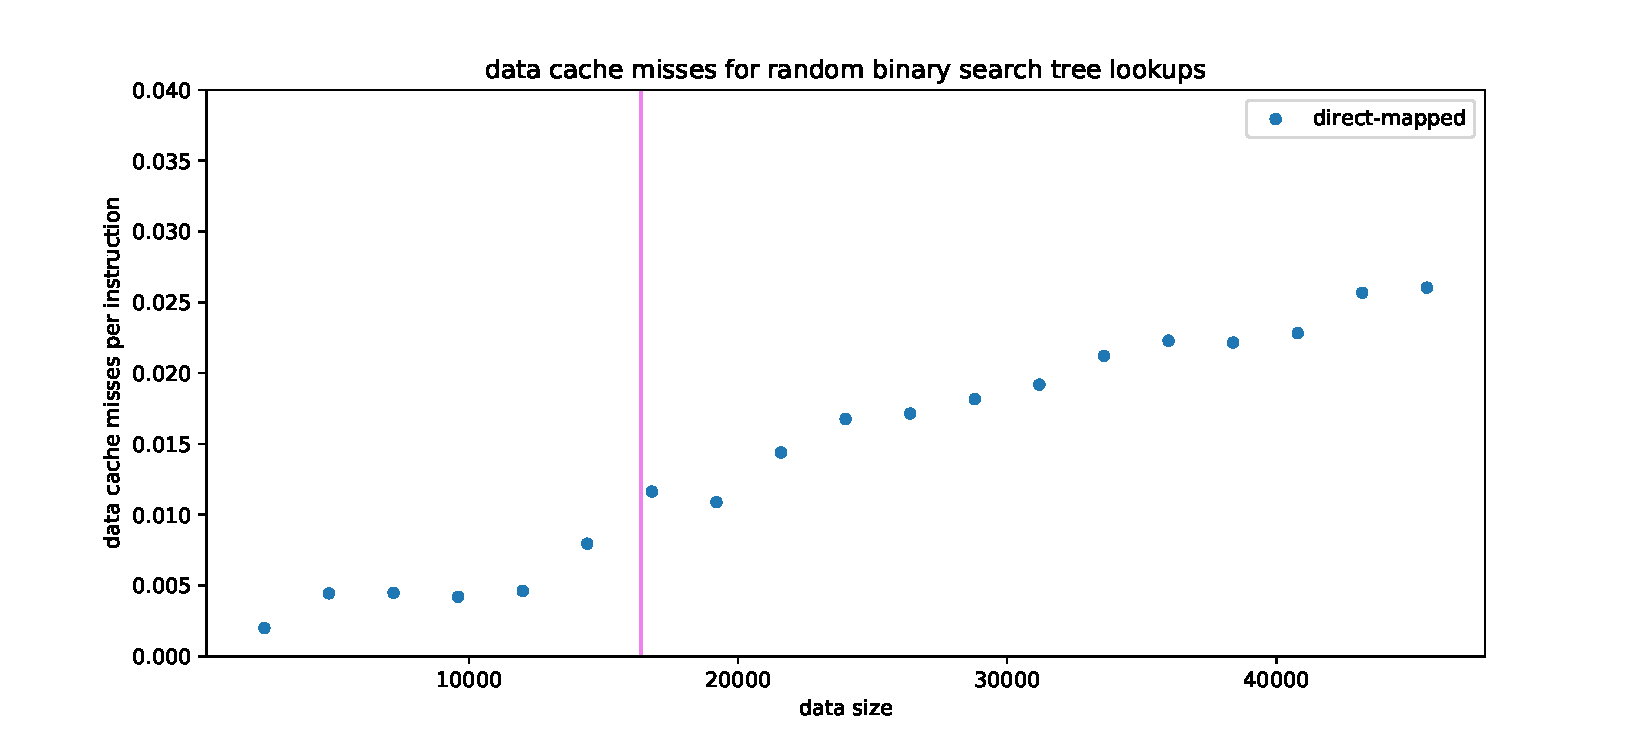
\includegraphics[width=\textwidth]{../caching/bst-one}
(simulated 16KB direct-mapped data cache; excluding BST setup)
\end{frame}

\begin{frame}{actual misses: BST lookups}
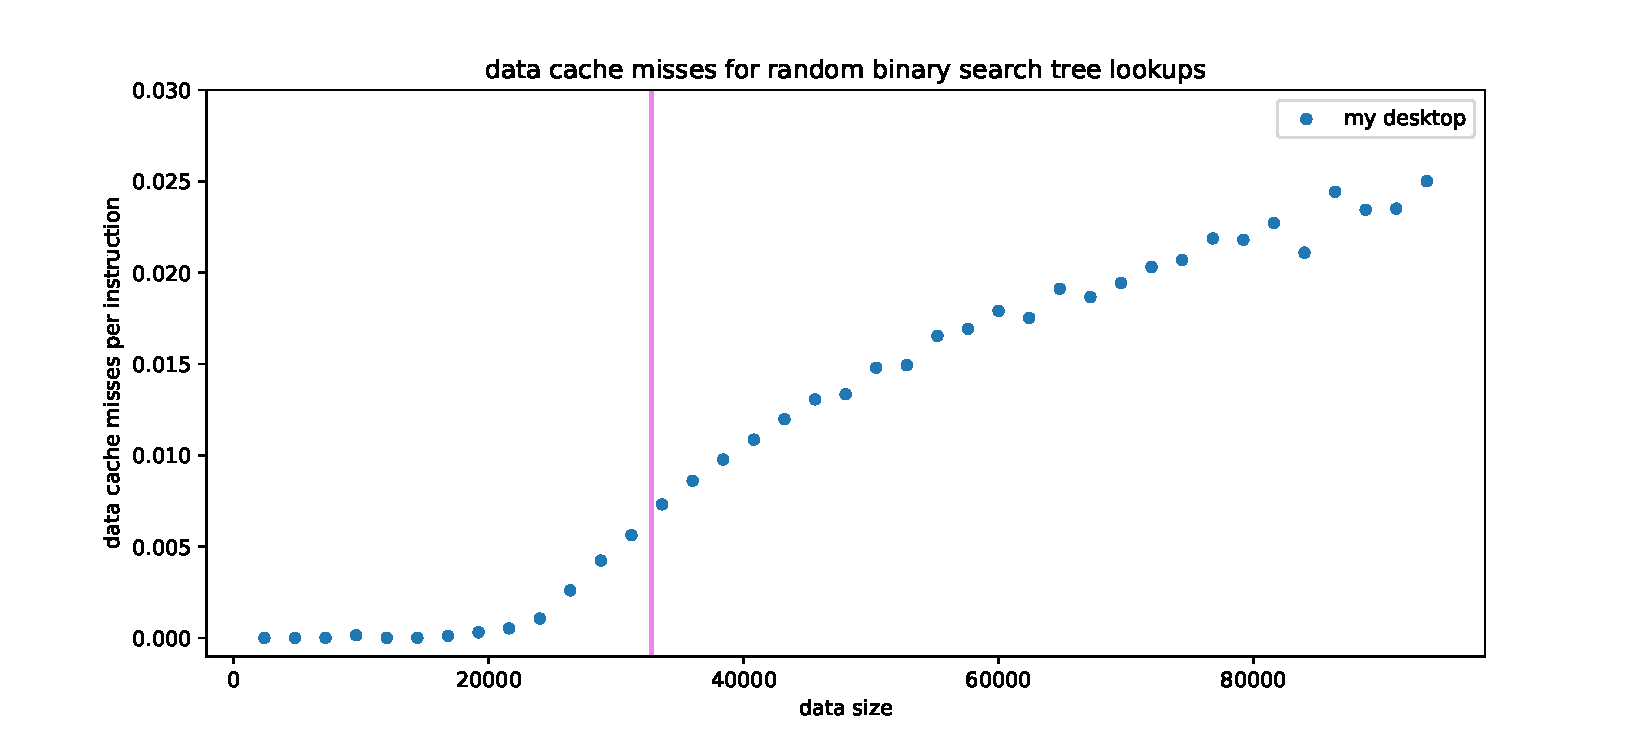
\includegraphics[width=\textwidth]{../caching/bst-act}
(actual 32KB more complex data cache) \\
\small (only one set of measurements + other things on machine + excluding initial load)
\end{frame}


\begin{frame}{simulated misses: matrix multiplies}
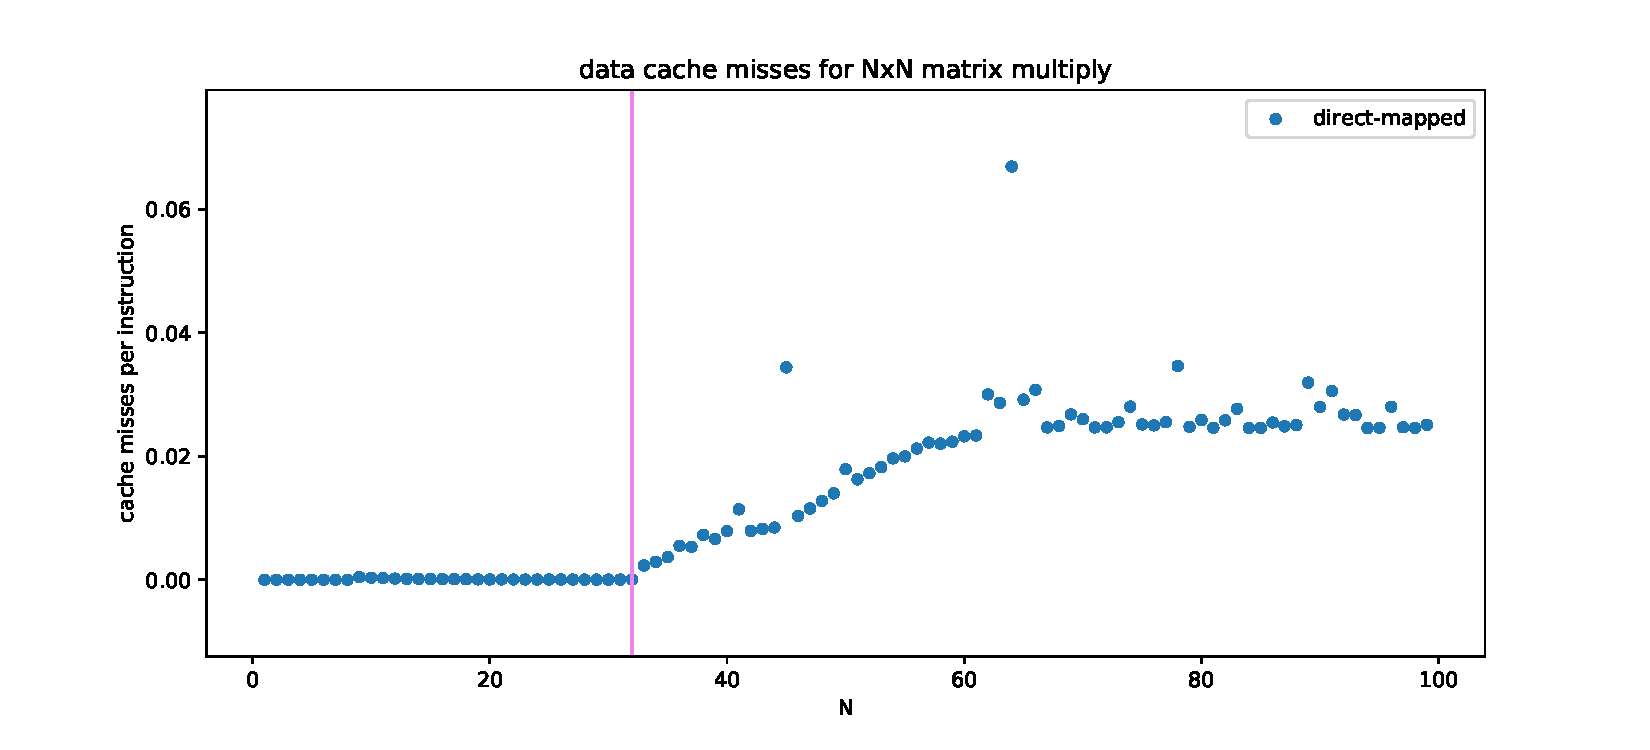
\includegraphics[width=\textwidth]{../caching/mm-one}
(simulated 16KB direct-mapped data cache; excluding initial load)
\end{frame}

\begin{frame}{actual misses: matrix multiplies}
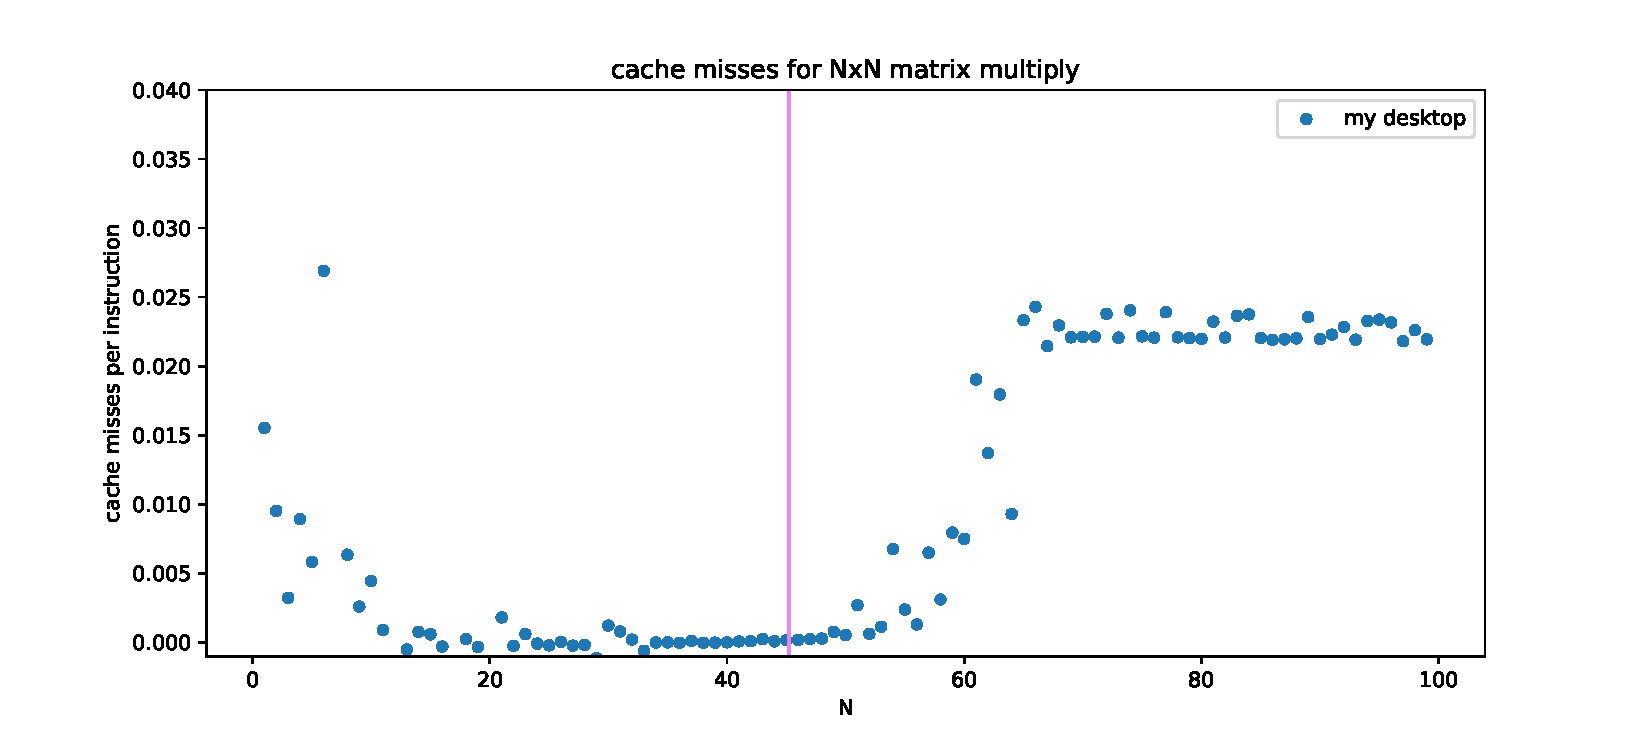
\includegraphics[width=\textwidth]{../caching/mm-act}
(actual 32KB more complex data cache; excluding matrix initial load) \\
\small (only one set of measurements + other things on machine)
\end{frame}


\section{adding associativity}
\usetikzlibrary{arrows.meta,calc,fit,positioning,matrix,circuits.logic.US,shapes.callouts}
\usetikzlibrary{circuits.logic.mux}
\begin{frame}<1-3,12,4->[fragile,label=assocPattern]{adding associativity}
\tikzset{
    v/.style={visible on=<#1->,alt=<#1>{red}},
    h/.style={alt=<#1>{red}},
    tagColor/.style={color=green!60!black},
    dataColor/.style={color=blue!60!black},
    offsetColor/.style={color=yellow!30!black},
}

\begin{tikzpicture}
\matrix[tight matrix,
        nodes={font=\small\tt,text depth=.1ex,text height=1ex,minimum height=1cm},
        row 1/.append style={nodes={font=\small\bfseries,minimum height=.5cm}},
        column 1/.append style={nodes={draw=none,text width=1.2cm}},
        column 2/.append style={nodes={align=center,text width=1cm}},
        column 3/.append style={nodes={align=center,tagColor,text width=1.5cm}},
        column 4/.append style={nodes={text width=2.5cm,align=center,dataColor,
            text depth=2.3ex}},
        column 5/.append style={nodes={draw=none,text width=.1cm}},
        column 6/.append style={nodes={align=center,text width=1cm}},
        column 7/.append style={nodes={align=center,tagColor,text width=1.5cm}},
        column 8/.append style={nodes={text width=2.5cm,align=center,dataColor,
            text depth=2.3ex}},
        row 1 column 4/.append style={nodes={text depth=.1ex}},
        row 1 column 8/.append style={nodes={text depth=.1ex}},
        label={[font=\small]$2$-way set associative, $2$ byte blocks, $2$ sets}] (cache)  {
index \& valid \& tag \& value \& ~ \& valid \& tag \& value \\
0\&
    % i 0, 0:
    \zzx{1}{4}{0}\z{5}{1} \& 
    \z{5}{000000} \& 
    \z{5}{mem[0x00] mem[0x01]}  \& ~ \&
    % i 0, 1:
    \zzx{1}{7}{0}\z{8}{1} \& 
    \z{8}{011000} \& 
    \z{8}{mem[0x60] mem[0x61]} \\
1\& 
    % i 1, 0:
    \zzx{1}{6}{0}\z{7}{1} \& 
    \z{7}{011000} \&
    \z{7}{mem[0x62] mem[0x63]} \& ~ \&
    % i 1, 1:
    0 \& ~ \& ~ \\
};

\begin{visibleenv}<1|handout:0>
    \node[below=1cm of cache,align=left,draw=red,very thick] {
        multiple places to put values with same index \\
        avoid misses from two active values using same set \\
        (``conflict misses''))
    };
\end{visibleenv}

\begin{visibleenv}<5-|handout:2>
    \matrix[tight matrix,anchor=north west,
            nodes={font=\small,minimum height=.5cm,text depth=.1ex},
            column 1/.append style={nodes={font=\small\tt,text width=3.3cm,align=left}},
            row 1/.append style={nodes={font=\small\bfseries}},
            column 2/.append style={nodes={text width=1.3cm}},
            ] (pattern) at ([yshift=-.5cm]cache.south west) {
        address (hex)\& result \\
        00000000 (00) \& |[v=5]| miss \\
        00000001 (01) \& |[v=6]| hit \\
        01100011 (63) \& |[v=7]| miss \\
        01100001 (61) \& |[v=8]| miss \\
        01100010 (62) \& |[v=9]| hit \\
        00000000 (00) \& |[v=10]| hit \\
        01100100 (64) \& |[v=11]| miss \\
    };
    \coordinate (tagTopLeft) at ([xshift=.1ex]pattern-2-1.north west);
    \coordinate (tagBottomLeft) at ([xshift=.1ex]pattern-8-1.south west);
    \coordinate (indexTopLeft) at ([xshift=6\oneZero]tagTopLeft);
    \coordinate (offsetTopLeft) at ([xshift=1\oneZero]indexTopLeft);
    \coordinate (offsetTopRight) at ([xshift=1\oneZero]offsetTopLeft);
    \coordinate (tagBottomRight) at (tagBottomLeft -| indexTopLeft);
    \coordinate (indexBottomRight) at (tagBottomLeft -| offsetTopLeft);
    \coordinate (offsetBottomRight) at (tagBottomLeft -| offsetTopRight);
    \fill[tagColor,opacity=0.3] (tagTopLeft) rectangle (tagBottomRight);
    \fill[offsetColor,opacity=0.3] (offsetTopLeft) rectangle (offsetBottomRight);
    \begin{scope}[every node/.style={anchor=north,text depth=.2ex,text height=1ex}]
        \node[tagColor,xshift=-.5cm] at ($(tagBottomLeft)!.5!(tagBottomRight)$) {
            tag
        };
        \node[xshift=-.2cm] at ($(tagBottomRight)!.5!(indexBottomRight)$) {
            index
        };
        \node[offsetColor,xshift=.6cm] at ($(indexBottomRight)!.5!(offsetBottomRight)$) {
            offset
        };
    \end{scope}
\end{visibleenv}

\begin{visibleenv}<11>
    \node[my callout2=pattern-8-2.east,anchor=west] at ([xshift=-1cm,yshift=1.2cm]pattern-8-2.east) { 
        needs to replace block in set 0!
    };
    \node[inner sep=-1pt,draw=red,line width=2pt,fit=(cache-2-2) (cache-2-8)] {};
\end{visibleenv}

\begin{visibleenv}<2>
    \node[inner sep=-1pt,draw=red,line width=2pt,fit=(cache-2-2) (cache-2-8),
        label={[red,xshift=-1cm,font=\bfseries]center:set 0}] {};
    \node[inner sep=-1pt,draw=red,line width=2pt,fit=(cache-3-2) (cache-3-8),
        label={[red,xshift=-1cm,font=\bfseries]center:set 1}] {};
\end{visibleenv}

\begin{visibleenv}<3>
    \node[inner sep=-1pt,draw=orange,line width=2pt,fit=(cache-2-2) (cache-3-4),
        label={[orange,font=\bfseries,fill=white]center:way 0}] {};
    \node[inner sep=-1pt,draw=orange,line width=2pt,fit=(cache-2-6) (cache-3-8),
        label={[orange,font=\bfseries,fill=white]center:way 1}] {};
\end{visibleenv}

\begin{visibleenv}<4|handout:2>
    \node[anchor=north west,font=\small,align=left] (explain1) at ([yshift=-.5cm]cache.south west) {
        $m = 8$ bit addresses \\ 
        $S=2=2^s$ sets \\
        $s=\myemph<2>{1}$ (set) index bits \\
    };
    \node[anchor=north west,font=\small,align=left] (explain2) at ([xshift=.5cm]explain1.north east) {
        $B=2=2^b$ byte block size \\
        $b=\myemph<2>{1}$ (block) offset bits \\
        $t = m - (s+b) = \myemph<2>{6}$ tag bits\\
    };
\end{visibleenv}

\end{tikzpicture}
\end{frame}

\begin{frame}{cache operation (associative)}
\begin{tikzpicture}[circuit logic US]
\tikzset{
    myline/.style={-latex,thick},
    myline thin/.style={-latex,thin},
    myline bus/.style={-latex,ultra thick},
    myline no arrow/.style={thick},
    offsetColor/.style={color=yellow!30!black},
    tagColor/.style={color=green!60!black},
    tagStoreFill/.style={fill=green!20},
    tagColorFill/.style={tagColor,fill=green!60!black},
    dataColor/.style={color=blue!60!black},
    dataColorFill/.style={tagColor,fill=blue!60!black},
    dataStoreFill/.style={fill=blue!20},
    triangle down/.style = {draw,regular polygon, regular polygon sides=3, shape border rotate=180},
}
\matrix[tight matrix,
        nodes={draw,
               font=\small\tt,
               text depth=0.2ex,
               text height=1.4ex,
        },
        row 1/.style={nodes={font=\small\bfseries}},
        column 1/.style={nodes={text width=1cm,align=center}},
        column 2/.style={nodes={text width=1cm,tagColor,tagStoreFill}},
        column 3/.style={nodes={text width=1.3cm,dataColor,dataStoreFill}},
        column 4/.style={nodes={text width=.1cm,draw=none}},
        column 5/.style={nodes={text width=1cm,align=center}},
        column 6/.style={nodes={text width=1cm,tagColor,tagStoreFill}},
        column 7/.style={nodes={text width=1.3cm,dataColor,dataStoreFill}},
        ] (cache) {
    valid \& tag \&  data \& ~ \& valid \& tag \& data\\
    1  \& 10 \& 00 11 \& ~ \& 1 \& 00 \& AA BB \\
    ~ \& ~ \& ~ \&   ~ \&  ~ \& ~ \& ~\\
    ~ \& ~ \& ~ \&   ~ \&  ~ \& ~ \& ~\\
    ~ \& ~ \& ~ \&   ~ \&  ~ \& ~ \& ~\\
    1 \&  11 \& B4 B5 \& ~ \& 1 \& 01 \& 33 44 \\
    ~ \& ~ \& ~ \&   ~ \&  ~ \& ~ \& ~\\
    ~ \& ~ \& ~ \&   ~ \&  ~ \& ~ \& ~\\
    ~ \& ~ \& ~ \&   ~ \&  ~ \& ~ \& ~\\
};
\begin{scope}[every node/.style={draw,rectangle,dashed,inner xsep=0pt,outer sep=0pt,font=\tt}]
\node (idx) at ([yshift=.5cm,xshift=-.3cm]cache.north west){100};
\node[left=0cm of idx,tagColor] (tag) {11};
\node[right=0cm of idx,offsetColor] (offset) {1};
\end{scope}
\draw[thick,dashed,-latex] (idx) |- (cache-6-1.west) node[near start,font=\small,fill=white,inner sep=2pt,xshift=-.3cm] {index};

%\begin{visibleenv}<2->
    \node[below=0.3cm of cache-9-2,draw,circle,inner sep=3pt] (comp1) {\small =};
    \node[below=1.4cm of cache-9-6,draw,circle,inner sep=3pt] (comp2) {\small =};
    %\coordinate(comp1Intersect) at ($(comp1) + (-.7cm,0.5cm)$);
    %\node[draw,circle,tagColorFill,inner sep=0pt,minimum width=1mm] at (comp1Intersect) {};
    \draw[tagColor,myline] (cache-9-2) -- (comp1);
    \draw[tagColor,myline] (cache-9-6) -- (comp2);

    %\draw[myline no arrow,tagColor] (tag) |- (comp1Intersect);
    %\draw[myline,tagColor] (comp1Intersect) |- (comp1);
    \draw[tagColor,myline] (tag) |- (comp2);
    \draw[tagColor,myline] (tag) |- (comp1) node[near start,font=\small,fill=white] {tag};
    %\draw[myline no arrow,tagColor] (comp1Intersect) |- (comp2Intersect);
    %\draw[myline,tagColor] (comp2Intersect) |- (comp2);

    \node[xshift=-.4cm,draw,below=1cm of cache-9-3,and gate,logic gate inputs=nn,label={[font=\scriptsize]center:AND}] (validCheck1) {};
    \node[xshift=-.4cm,draw,below=2.0cm of cache-9-7,and gate,logic gate inputs=nn,label={[font=\scriptsize]center:AND}] (validCheck2) {};
    \draw[myline] (comp1.south) |- (validCheck1.input 1);
    \draw[myline] (cache-9-1.south) |- (validCheck1.input 2);
    \draw[myline] (comp2.south) |- (validCheck2.input 1);
    \draw[myline] (cache-9-5.south) |- (validCheck2.input 2);
%\end{visibleenv}

\node[fit=(cache-6-1) (cache-6-7),inner sep=1pt,red,draw,line width=3pt] {};

%\node[draw,trapezium,inner xsep=0pt,outer sep=0pt,trapezium angle=75,below=.7cm of validCheck2,
%text width=5cm,shape border rotate=180,xshift=1.5cm] (mux) {};
%\draw[myline] (validCheck1.output) -| (buffer1.west);
%\draw[myline] (cache-9-3.south) -- (buffer1);
%\draw[myline] (buffer1.south) -- (bufEnd1);
\coordinate (outputData) at ([xshift=1.5cm,yshift=-.5cm]cache-9-7.south east);
\coordinate (beforeOutputData) at ([xshift=-.5cm]outputData);
\coordinate (outputHit1) at ([xshift=-1.5cm] beforeOutputData |- validCheck1.output);
\coordinate (outputHit2) at ([xshift=-1.5cm] beforeOutputData |- validCheck2.output);
%\begin{visibleenv}<2->
\node[or gate,logic gate inputs=nn,label={[font=\scriptsize]center:OR},anchor=output] (validCheckTotal)
    at ([xshift=1cm]$(outputHit1)!0.5!(outputHit2)$) {};
%\draw[myline] (validCheck1.output) -- (outputHit1) |- (validCheckTotal.input 1);
    \draw[myline no arrow] (validCheck1.output) -- ([xshift=-1pt]validCheck1.output -| cache-9-5.south);
    \draw[myline no arrow] ([xshift=1pt]validCheck1.output -| cache-9-5.south) -- 
                  ([xshift=-2pt]validCheck1.output -| cache-9-6.south);
    \draw[myline no arrow] ([xshift=2pt]validCheck1.output -| cache-9-6.south) -- (outputHit1);
    \draw[myline] (outputHit1) |- (validCheckTotal.input 1);
\draw[myline] (validCheck2.output) -- (outputHit2) |- (validCheckTotal.input 2);
\draw[myline] (validCheckTotal.output) -- ++(.5cm,0cm) node[right] {is hit? ({\tt 1})};
%\end{visibleenv}
%\begin{visibleenv}<3->
    \node[dataColor,draw,minimum width=.5cm,minimum height=1cm,mux,anchor=east,inputs=nn] (outputSelect) at ([xshift=-.2cm]beforeOutputData) {};
    \draw[myline] (outputHit1) -| (outputSelect.south);
    \fill[black] (outputHit1) circle (2pt);
    %\draw[myline,dataColor] (cache-9-3.south) |- (outputSelect.input 2);
        \draw[dataColor,myline no arrow] (cache-9-3.south) |- ([xshift=-1pt]cache-9-5.south |- outputSelect.input 2);
        \draw[dataColor,myline no arrow] ([xshift=1pt]cache-9-5.south |- outputSelect.input 2) --
                               ([xshift=-1pt]cache-9-6.south |- outputSelect.input 2);
        \draw[dataColor,myline] ([xshift=1pt]cache-9-6.south |- outputSelect.input 2) --
                               (outputSelect.input 2);
    \draw[myline,dataColor] (cache-9-7.south) |- (outputSelect.input 1);
    \draw[myline no arrow,dataColor] (outputSelect.output) -- (beforeOutputData);
    \node[draw,minimum width=.5cm,minimum height=1cm,mux,anchor=west,inputs=nn] (selectByte) at (outputData) {};
    \foreach \x in {1,2} {
        \draw[dataColor,myline thin] (beforeOutputData) |- (selectByte.input \x);
    };
    \draw[offsetColor,myline] (offset.east) -| (selectByte.north) node[very near start,fill=white,font=\small] {offset};
    \draw[dataColor,myline thin] (selectByte.output) -- ++(0.5cm,0cm) -- ++(0cm,0.5cm) node[above,align=center] {data\\({\tt B5})};
%\end{visibleenv}

\begin{visibleenv}<2-3>
\node[draw,red,thick,fit=(validCheck1)] {};
\node[draw,red,thick,fit=(comp1)] {};
\draw[red,thick,dashed,-Latex] (validCheck1.output) -| (outputSelect.south);
\end{visibleenv}
\begin{visibleenv}<3>
\draw[thick,red,-Latex] (outputSelect.input 2) -- (outputSelect.output);
\end{visibleenv}
\end{tikzpicture}
% FIXME: place diagram here
\end{frame}

% FIXME: drop slide?
\begin{frame}{associative lookup possibilities}
    \begin{itemize}
    \item none of the blocks for the index are valid
    \item none of the valid blocks for the index match the tag
        \begin{itemize}
        \item something else is stored there
        \end{itemize}
    \item one of the blocks for the index is valid and matches the tag
    \end{itemize}
\end{frame}


\subsection{diagram}
\usetikzlibrary{decorations,decorations.pathreplacing,circuits.logic.US,matrix,positioning,fit}
\usetikzlibrary{circuits.logic.mux}

\begin{frame}{cache operation (associative)}
\begin{tikzpicture}[circuit logic US]
\tikzset{
    myline/.style={-latex,thick},
    myline thin/.style={-latex,thin},
    myline bus/.style={-latex,ultra thick},
    myline no arrow/.style={thick},
    offsetColor/.style={color=yellow!30!black},
    tagColor/.style={color=green!60!black},
    tagStoreFill/.style={fill=green!20},
    tagColorFill/.style={tagColor,fill=green!60!black},
    dataColor/.style={color=blue!60!black},
    dataColorFill/.style={tagColor,fill=blue!60!black},
    dataStoreFill/.style={fill=blue!20},
    triangle down/.style = {draw,regular polygon, regular polygon sides=3, shape border rotate=180},
}
\matrix[tight matrix,
        nodes={draw,
               font=\small\tt,
               text depth=0.2ex,
               text height=1.4ex,
        },
        row 1/.style={nodes={font=\small\bfseries}},
        column 1/.style={nodes={text width=1cm,align=center}},
        column 2/.style={nodes={text width=1cm,tagColor,tagStoreFill}},
        column 3/.style={nodes={text width=1.3cm,dataColor,dataStoreFill}},
        column 4/.style={nodes={text width=.1cm,draw=none}},
        column 5/.style={nodes={text width=1cm,align=center}},
        column 6/.style={nodes={text width=1cm,tagColor,tagStoreFill}},
        column 7/.style={nodes={text width=1.3cm,dataColor,dataStoreFill}},
        ] (cache) {
    valid \& tag \&  data \& ~ \& valid \& tag \& data\\
    1  \& 10 \& 00 11 \& ~ \& 1 \& 00 \& AA BB \\
    ~ \& ~ \& ~ \&   ~ \&  ~ \& ~ \& ~\\
    ~ \& ~ \& ~ \&   ~ \&  ~ \& ~ \& ~\\
    ~ \& ~ \& ~ \&   ~ \&  ~ \& ~ \& ~\\
    1 \&  11 \& B4 B5 \& ~ \& 1 \& 01 \& 33 44 \\
    ~ \& ~ \& ~ \&   ~ \&  ~ \& ~ \& ~\\
    ~ \& ~ \& ~ \&   ~ \&  ~ \& ~ \& ~\\
    ~ \& ~ \& ~ \&   ~ \&  ~ \& ~ \& ~\\
};
\begin{scope}[every node/.style={draw,rectangle,dashed,inner xsep=0pt,outer sep=0pt,font=\tt}]
\node (idx) at ([yshift=1cm,xshift=-.3cm]cache.north west){100};
\node[left=0cm of idx,tagColor] (tag) {11};
\node[right=0cm of idx,offsetColor] (offset) {1};
\end{scope}
\draw[thick,dashed,-latex] (idx) |- ([xshift=-.2cm]cache-6-1.north west) node[near start,font=\small,fill=white,inner sep=2pt,xshift=-.3cm] {index};
\draw[very thick,decorate,decoration={brace,mirror},overlay] ([xshift=-.1cm]cache-2-1.north west) -- ([xshift=-.1cm]cache-9-1.south west);

\node[fit=(cache-6-1) (cache-6-7),inner sep=1pt,red,draw,line width=3pt] {};

\draw[thick,dashed,-latex,tagColor] (tag) |- ([yshift=-.5cm]cache-9-2.south) coordinate (tag cmp 1);
\draw[thick,dashed,-latex,tagColor] (cache-9-2.south) -- (tag cmp 1);
\draw[thick,dashed,-latex,tagColor] (tag) |- ([yshift=-1cm]cache-9-6.south) coordinate (tag cmp 2)
    node[pos=0.25,fill=white] {tag};
\draw[thick,dashed,-latex,tagColor] (cache-9-6.south) -- (tag cmp 2);

\draw[thick,dashed,-latex,offsetColor] (offset.south) -- ++(0cm, -.1cm) -| ([yshift=.2cm]cache-1-3.north);
\draw[thick,dashed,-latex,offsetColor] (offset.south) -- ++(0cm, -.1cm) -| ([yshift=.2cm]cache-1-7.north);

\draw[very thick,decorate,decoration={brace,mirror},overlay] ([yshift=.1cm]cache-1-3.north east) -- ([yshift=.1cm]cache-1-3.north west);
\draw[very thick,decorate,decoration={brace,mirror},overlay] ([yshift=.1cm]cache-1-7.north east) -- ([yshift=.1cm]cache-1-7.north west);

\end{tikzpicture}
% FIXME: place diagram here
\end{frame}


\subsection{options for replacement}
\usetikzlibrary{arrows.meta,calc,fit,matrix,positioning,shapes.callouts}
\begin{frame}[fragile,label=replPolicies]{replacement policies}
\tikzset{
    v/.style={visible on=<#1->,alt=<#1>{red}},
    h/.style={alt=<#1>{red}},
    tagColor/.style={color=green!60!black},
    dataColor/.style={color=blue!60!black},
    offsetColor/.style={color=yellow!30!black},
}

\begin{tikzpicture}
\matrix[tight matrix,
        nodes={font=\small\tt,text depth=.1ex,text height=1ex,minimum height=1cm},
        row 1/.append style={nodes={font=\small\bfseries,minimum height=.5cm}},
        column 1/.append style={nodes={draw=none,text width=1.1cm}},
        column 2/.append style={nodes={align=center,text width=1cm}},
        column 3/.append style={nodes={align=center,tagColor,text width=1.3cm,
            font=\tt\fontsize{10}{11}\selectfont}},
        column 4/.append style={nodes={text width=1.9cm,align=center,dataColor,
            font=\tt\fontsize{10}{11}\selectfont,
            text depth=2.3ex}},
        column 5/.append style={nodes={draw=none,text width=.1cm}},
        column 6/.append style={nodes={align=center,text width=1cm}},
        column 7/.append style={nodes={align=center,tagColor,text width=1.3cm,
            font=\tt\fontsize{10}{11}\selectfont}},
        column 8/.append style={nodes={text width=1.9cm,align=center,dataColor,
            font=\tt\fontsize{10}{11}\selectfont,
            text depth=2.3ex}},
        column 9/.append style={nodes={draw=none,text width=.1cm}},
        row 1 column 4/.append style={nodes={text depth=.1ex}},
        row 1 column 8/.append style={nodes={text depth=.1ex}},
        column 10/.append style={nodes={visible on=<2->,align=center}},
        label={[font=\small]$2$-way set associative, $2$ byte blocks, $2$ sets}] (cache)  {
index \& valid \& tag \& value \& ~ \& valid \& tag \& value \& ~\& LRU\\
0\&
    % i 0, 0:
    1 \& 
    000000 \& 
    mem[0x00] mem[0x01] \& ~\&
    % i 0, 1:
    1 \& 
    011000 \& 
    mem[0x60] mem[0x61] \& ~ \& 1 \\
1\& 
    % i 1, 0:
    1 \& 
    011000 \&
    mem[0x62] mem[0x63] \&  ~ \&
    % i 1, 1:
    0 \& ~ \& ~ \&  ~\& 1
    \\
};
\matrix[tight matrix,anchor=north west,
            nodes={font=\small,minimum height=.5cm,text depth=.1ex},
            column 1/.append style={nodes={font=\small\tt,text width=3.3cm,align=left}},
            row 1/.append style={nodes={font=\small\bfseries}},
            column 2/.append style={nodes={text width=1.3cm}},
            ] (pattern) at ([yshift=-.5cm]cache.south west) {
        address (hex)\& result \\
        00000000 (00) \&  miss \\
        00000001 (01) \& hit \\
        01100011 (63) \& miss \\
        01100001 (61) \& miss \\
        01100010 (62) \&  hit \\
        00000000 (00) \& hit \\
        01100100 (64) \& |[red]| miss \\
    };
\node[inner sep=-1pt,draw=red,line width=2pt,fit=(cache-2-2) (cache-2-8)] {};
\begin{visibleenv}<1|handout:0>
    \node[my callout2=cache-2-4.south,anchor=north] at ([yshift=-2cm]cache-2-4.south) {
        how to decide where to insert 0x64?
    };
\end{visibleenv}
\begin{visibleenv}<2>
    \node[my callout2=cache-3-10.south,anchor=north,align=left] at ([yshift=-1cm,xshift=-1cm]cache-3-8.south) {
        track which block was read least recently \\
        updated on \myemph{every access}
    };
\end{visibleenv}
\end{tikzpicture}
\end{frame}

\begin{frame}{example replacement policies}
\begin{itemize}
    \item least recently used
        \begin{itemize}
        \item take advantage of \myemph{temporal locality}
        \item at least $\left\lceil\log_2(E!)\right\rceil$ bits per set for $E$-way cache
            \begin{itemize}
            \item (need to store order of all blocks)
            \end{itemize}
        \end{itemize}
    \item approximations of least recently used
        \begin{itemize}
        \item implementing least recently used is expensive 
            \begin{itemize}
            \item lots of bookkeeping bits+time
            \end{itemize}
        \item really just need ``avoid recently used'' --- much faster/simpler
        \item good approximations: $E$ to $2E$ bits
        \end{itemize}
    \item first-in, first-out
        \begin{itemize}
        \item counter per set --- where to replace next
        \end{itemize}
    \item (pseudo-)random
        \begin{itemize}
        \item no extra information!
        \item actually works pretty well in practice
        \end{itemize}
\end{itemize}
\end{frame}



\usetikzlibrary{matrix,fit}
\begin{frame}[fragile,label=lruTrack]{LRU bit updating}
\tikzset{
    v/.style={visible on=<#1->,alt=<#1>{red}},
    h/.style={alt=<#1>{red}},
    tagColor/.style={color=green!60!black},
    dataColor/.style={color=blue!60!black},
    offsetColor/.style={color=yellow!30!black},
}

\begin{tikzpicture}
\matrix[tight matrix,
        nodes={font=\small\tt,text depth=.1ex,text height=1ex,minimum height=1cm},
        row 1/.append style={nodes={font=\small\bfseries,minimum height=.5cm}},
        column 1/.append style={nodes={draw=none,text width=1.1cm}},
        column 2/.append style={nodes={align=center,text width=1cm}},
        column 3/.append style={nodes={align=center,tagColor,text width=1.3cm,
            font=\tt\fontsize{10}{11}\selectfont}},
        column 4/.append style={nodes={text width=1.9cm,align=center,dataColor,
            font=\tt\fontsize{10}{11}\selectfont,
            text depth=2.3ex}},
        column 5/.append style={nodes={draw=none,text width=.1cm}},
        column 6/.append style={nodes={align=center,text width=1cm}},
        column 7/.append style={nodes={align=center,tagColor,text width=1.3cm,
            font=\tt\fontsize{10}{11}\selectfont}},
        column 8/.append style={nodes={text width=1.9cm,align=center,dataColor,
            font=\tt\fontsize{10}{11}\selectfont,
            text depth=2.3ex}},
        column 9/.append style={nodes={draw=none,text width=.1cm}},
        row 1 column 4/.append style={nodes={text depth=.1ex}},
        row 1 column 8/.append style={nodes={text depth=.1ex}},
        column 10/.append style={nodes={visible on=<2->,align=center}},
        label={[font=\small]$2$-way set associative, $2$ byte blocks, $2$ sets}] (cache)  {
index \& valid \& tag \& value \& ~ \& valid \& tag \& value \& ~\& LRU\\
0\&
    % i 0, 0:
    \zzx{1}{7}{1}\z{8}{1} \& 
    \zzx{1}{7}{000000}\z{8}{111000} \& 
    \zzx{1}{7}{mem[0x00] mem[0x01]}\z{8}{mem[0xe0] mem[0xe1]} \& ~\&
    % i 0, 1:
    \z{2}{1} \& 
    \zz{2}{5}{011000}\z{6}{111100} \& 
    \zz{2}{5}{mem[0x60] mem[0x61]}\z{6}{mem[0xf0] mem[0xf1]} \& ~ \&
    \zzx{1}{1}{1}\zz{2}{3}{0}\zz{4}{5}{1}\zz{6}{7}{0}\z{8}{1} \\
1\& 
    % i 1, 0:
    1 \& 
    011000 \&
    mem[0x62] mem[0x63] \&  ~ \&
    % i 1, 1:
    0 \& ~ \& ~ \&  ~\& 1
    \\
};
\matrix[tight matrix,anchor=north west,
            nodes={font=\small,minimum height=.5cm,text depth=.1ex},
            column 1/.append style={nodes={font=\small\tt,text width=3.3cm,align=left}},
            row 1/.append style={nodes={font=\small\bfseries}},
            column 2/.append style={nodes={text width=1.3cm}},
            ] (pattern) at ([yshift=-.5cm]cache.south west) {
        address (hex)\& result \\
        \ldots \& \ldots \\
        01100001 (61) \& |[v=1]| miss \\
        01100000 (60) \& |[v=3]| hit \\
        01100000 (61) \& |[v=3]| hit \\
        00000000 (00) \& |[v=4]| hit \\
        11110000 (f0) \& |[v=5]| miss \\
        11100000 (e0) \& |[v=7]| miss \\
    };
\node[inner sep=-1pt,draw=red,line width=2pt,fit=(cache-2-2) (cache-2-8)] {};
    \coordinate (tagTopLeft) at ([xshift=.1ex]pattern-2-1.north west);
    \coordinate (tagBottomLeft) at ([xshift=.1ex]pattern-8-1.south west);
    \coordinate (indexTopLeft) at ([xshift=4\oneZero]tagTopLeft);
    \coordinate (offsetTopLeft) at ([xshift=2\oneZero]indexTopLeft);
    \coordinate (offsetTopRight) at ([xshift=2\oneZero]offsetTopLeft);
    \coordinate (tagBottomRight) at (tagBottomLeft -| indexTopLeft);
    \coordinate (indexBottomRight) at (tagBottomLeft -| offsetTopLeft);
    \coordinate (offsetBottomRight) at (tagBottomLeft -| offsetTopRight);
    \fill[tagColor,opacity=0.3] (tagTopLeft) rectangle (tagBottomRight);
    \begin{scope}[every node/.style={anchor=north,text depth=.2ex,text height=1ex}]
        \node[tagColor,xshift=-.5cm] at ($(tagBottomLeft)!.5!(tagBottomRight)$) {
            tag
        };
        \node[xshift=-.2cm] at ($(tagBottomRight)!.5!(indexBottomRight)$) {
            index
        };
        \node[offsetColor,xshift=.6cm] at ($(indexBottomRight)!.5!(offsetBottomRight)$) {
            offset
        };
    \end{scope}
\end{tikzpicture}
\end{frame}


\subsection{associativity terms}
\begin{frame}{associativity terminology}
\begin{itemize}
\item \myemph{direct-mapped} --- one block per set
\item \myemph{$E$-way set associative} --- $E$ blocks per set
    \begin{itemize}
    \item $E$ ways in the cache
    \end{itemize}
\item \myemph{fully associative} --- one set total (everything in one set)
\end{itemize}
\end{frame}


\subsection{tag/index/offset for set-assoc. caches}
\begin{frame}{Tag-Index-Offset formulas}
\def\arraystretch{1.5}
\begin{tabular}{ll}
$m$ & memory addreses bits \\
$E$ & number of blocks per set (``ways'') \\
$S=2^s$ & number of sets \\
$s$  & (set) index bits \\
$B=2^b$ & block size \\
$b$ & (block) offset bits \\
$t = m - (s+b)$ & tag bits \\
$C = B \times S \times E$ & cache size (excluding metadata) \\
\end{tabular}
\end{frame}


% FIXME: direct-mapped and C code example
\section{misses in C, and intuition behind conflicts}
\begin{frame}[fragile,label=accessesAndCCode]{cache accesses and C code (1)}
\begin{lstlisting}[style=small]
int scaleFactor;

int scaleByFactor(int value) {
    return value * scaleFactor;
}
\end{lstlisting}
\hrule
\begin{lstlisting}[language=myasm,style=small]
scaleByFactor:
    movl scaleFactor, %eax
    imull %edi, %eax
    ret
\end{lstlisting}
\hrule
\begin{itemize}
\item exericse: what data cache accesses does this function do?
    \begin{itemize}
    \item<2-> 4-byte read of scaleFactor
    \item<2-> 8-byte read of return address
    \end{itemize}
\end{itemize}
\end{frame}

\begin{frame}[fragile,label=sfUse]{possible scaleFactor use}
\begin{lstlisting}[style=small]
for (int i = 0; i < size; ++i) {
    array[i] = scaleByFactor(array[i]);
}
\end{lstlisting}
\end{frame}

\begin{frame}[fragile,label=conflictsAndCode]{misses and code (2)}
\begin{lstlisting}[language=myasm,style=smaller]
scaleByFactor:
    movl scaleFactor, %eax
    imull %edi, %eax
    ret
\end{lstlisting}
\begin{itemize}
\item suppose each time this is called in the loop:
    \begin{itemize}
    \item return address located at address \texttt{0x7ffffffe43b8}
    \item scaleFactor located at address \texttt{0x6bc3a0}
    \end{itemize}
\item with direct-mapped 32KB cache w/64 B blocks, what is their:
\begin{tabular}{l|l|l}
~ & return address & scaleFactor \\ \hline
tag &  \only<2->{0xfffffffc} & \only<2->{0xd7} \\
index & \only<2->{\myemph<3>{0x10e}} & \only<2->{\myemph<3>{0x10e}} \\
offset & \only<2->{0x38} & \only<2->{0x20} \\
\end{tabular}
\end{itemize}
\end{frame}

\begin{frame}{conflict miss coincidences?}
\begin{itemize}
\item obviously I set that up to have the same index 
    \begin{itemize}
    \item have to use exactly the right amount of stack space\ldots
    \end{itemize}
\item but one of the reasons we'll want something better
    than direct-mapped cache
\end{itemize}
\end{frame}


\subsection{array misses warmup}
\usetikzlibrary{decorations.pathreplacing,matrix}

\begin{frame}[fragile,label=arrayMissesWarmup1]{C and cache misses (warmup 1)}
\begin{lstlisting}
int array[4];
...
int even_sum = 0, odd_sum = 0;
even_sum += array[0];
odd_sum += array[1];
even_sum += array[2];
odd_sum += array[3];
\end{lstlisting}
\begin{itemize}
\item {\small
Assume everything but {\tt array} is kept in registers (and the compiler does not do
anything funny).}
\item How many data cache misses on a 1-set direct-mapped cache with 8B blocks?
\end{itemize}
\end{frame}

\begin{frame}<1>[fragile,label=arrayMissesWarmup1Answers]{some possiblities}
    \newcommand{\mywidth}{0.39}
\begin{tikzpicture}
    % FIXME: picture
        % array versus cache blocks layout
        % show each each block maps to array, with cache blocks lining up properly
    \foreach \offset in {-2,-1,0,1,2,...,31,32,33} {
        \draw[black!25,thin] (\offset * \mywidth, 0) rectangle ++(\mywidth, -1);
    }
    \node[font=\large,anchor=east] at (-2 * \mywidth, -.5) {\ldots};
    \node[font=\large,anchor=west] at (34 * \mywidth, -.5) {\ldots};
    \foreach \offset/\name in {8/0,12/1,16/2,20/3} {
        \draw[thin,fill=blue!10] (\offset * \mywidth, 0) rectangle ++(\mywidth * 4, -1)
            node[fill=none,opacity=1.0,black,midway,font=\fontsize{9}{10}\tt\selectfont] {array[\name]};
    }
    \begin{visibleenv}<1>
    \node[anchor=north west,align=left] at (0, -1.25) {
        Q1: how do cache blocks correspond to array elements? \\
        not enough information provided!
    };
    \end{visibleenv}
    \begin{visibleenv}<2>
    \node[anchor=north west,align=left] at (0, -1.25) {
        if array[0] starts at beginning of a cache block\ldots \\
        array split across two cache blocks
    };
    \begin{scope}
    \clip (-2.1 * \mywidth, .2) rectangle (34.1 * \mywidth, -1.1);
    \foreach \offset in {-8,0,8,16,24,32} {
        \draw[ultra thick,red!30!black] (\offset * \mywidth, 0)
            rectangle ++(\mywidth * 8, -1);
    }
    \end{scope}
        \draw[very thick, decorate, decoration={brace}] (16 * \mywidth, 0.05) -- ++(8 * \mywidth, 0)
            node[above,midway,overlay] {one cache block};
    \matrix[tight matrix,
        nodes={minimum height=0.7cm},
        column 1/.append style={nodes={text width=6cm}},
        column 2/.append style={nodes={text width=6cm,font=\tt}},
        row 1/.append style={nodes={font=\bfseries}},
        anchor=north west] at (0, -3) {
        memory access \& cache contents afterwards \\ 
        --- \& (empty) \\
        read \lstinline|array[0]| (miss) \& \{array[0], array[1]\} \\
        read \lstinline|array[1]| (hit) \& \{array[0], array[1]\} \\
        read \lstinline|array[2]| (miss) \& \{array[2], array[3]\} \\
        read \lstinline|array[3]| (hit) \& \{array[2], array[3]\} \\
    };
    \end{visibleenv}
    \begin{visibleenv}<3>
    \node[anchor=north west,align=left] at (0, -1.25) {
        if array[0] starts right in the middle of a cache block \\
        array split across three cache blocks
    };
    \begin{scope}
    \clip (-2.1 * \mywidth, .2) rectangle (34.1 * \mywidth, -1.1);
    \foreach \offset in {-4,4,12,20,28} {
        \draw[ultra thick,red!30!black] (\offset * \mywidth, 0)
            rectangle ++(\mywidth * 8, -1);
    }
    \end{scope}
        \draw[very thick, decorate, decoration={brace}] (12 * \mywidth, 0.05) -- ++(8 * \mywidth, 0)
            node[above,midway,overlay] {one cache block};
    \foreach \offset/\name in {4/****,24/++++} {
        \path (\offset * \mywidth, 0) rectangle ++(\mywidth * 4, -1)
            node[fill=none,opacity=1.0,black,midway,font=\fontsize{9}{10}\tt\selectfont] {\name};
    }
    \matrix[tight matrix,
        nodes={minimum height=0.7cm},
        column 1/.append style={nodes={text width=6cm}},
        column 2/.append style={nodes={text width=6cm,font=\tt}},
        row 1/.append style={nodes={font=\bfseries}},
        anchor=north west] at (0, -3) {
        memory access \& cache contents afterwards \\ 
        --- \& (empty) \\
        read \lstinline|array[0]| (miss) \& \{****, array[0]\} \\
        read \lstinline|array[1]| (miss) \& \{array[1], array[2]\} \\
        read \lstinline|array[2]| (hit) \& \{array[1], array[2]\} \\
        read \lstinline|array[3]| (miss) \& \{array[3], ++++\} \\
    };
    \end{visibleenv}
    \begin{visibleenv}<4>
    \node[anchor=north west,align=left] at (0, -1.25) {
        if array[0] starts at an odd place in a cache block, \\
        need to read two cache blocks to get most array elements
    };
    \begin{scope}
    \clip (-2.1 * \mywidth, .2) rectangle (34.1 * \mywidth, -1.1);
    \foreach \offset in {-7,1,9,17,25,33} {
        \draw[ultra thick,red!30!black] (\offset * \mywidth, 0)
            rectangle ++(\mywidth * 8, -1);
    }
    \end{scope}
        \draw[very thick, decorate, decoration={brace}] (9 * \mywidth, 0.05) -- ++(8 * \mywidth, 0)
            node[above,midway,overlay] {one cache block};
    \foreach \offset/\name in {4/****,24/++++} {
        \path (\offset * \mywidth, 0) rectangle ++(\mywidth * 4, -1)
            node[fill=none,opacity=1.0,black,midway,font=\fontsize{9}{10}\tt\selectfont] {\name};
    }
    \matrix[tight matrix,
        nodes={minimum height=0.5cm},
        column 1/.append style={nodes={text width=6cm,font=\small}},
        column 2/.append style={nodes={text width=6cm,align=center,font=\fontsize{8}{9}\selectfont}},
        row 1/.append style={nodes={font=\bfseries}},
        anchor=north west] at (0, -3) {
        memory access \& cache contents afterwards \\ 
        --- \& (empty) \\
        read \lstinline|array[0]| byte 0 (miss) \& \{ ****, array[0] byte 0 \} \\
        read \lstinline|array[0]| byte 1-3 (miss) \& \{ array[0] byte 1-3, array[2], array[3] byte 0 \} \\
        read \lstinline|array[1]| (hit) \&  \{ array[0] byte 1-3, array[2], array[3] byte 0 \} \\
        read \lstinline|array[2]| byte 0 (hit) \& \{ array[0] byte 1-3, array[2], array[3] byte 0 \} \\
        read \lstinline|array[2]| byte 1-3 (miss) \& \{part of array[2], array[3], ++++\} \\
        read \lstinline|array[3]| (hit) \& \{part of array[2], array[3], ++++\} \\
    };
    \end{visibleenv}
\end{tikzpicture}
\end{frame}

\iftoggle{heldback}{}{
\againframe<2>{arrayMissesWarmup1Answers}
\againframe<3>{arrayMissesWarmup1Answers}
\againframe<4>{arrayMissesWarmup1Answers}
}

\begin{frame}{aside: alignment}
    \begin{itemize}
    \item compilers and malloc/new implementations usually try \myemph{align} values
    \item align = make address be multiple of something
    \vspace{.5cm}
    \item most important reason: don't cross cache block boundaries
    \end{itemize}
\end{frame}

\begin{frame}[fragile,label=arrayMissesWarmup2]{C and cache misses (warmup 2)}
\begin{lstlisting}
int array[4];
int even_sum = 0, odd_sum = 0;
even_sum += array[0];
even_sum += array[2];
odd_sum += array[1];
odd_sum += array[3];
\end{lstlisting}
\begin{itemize}
\item {\small
Assume everything but {\tt array} is kept in registers (and the compiler does not do
anything funny).}
\item Assume array[0] at beginning of cache block.
\item How many data cache misses on a 1-set direct-mapped cache with 8B blocks?
\end{itemize}
\end{frame}

\begin{frame}<0>[fragile,label=arrayMissesWarmup2Answers]{exercise solution}
    \newcommand{\mywidth}{0.39}
\begin{tikzpicture}
    \foreach \offset in {-2,-1,0,1,2,...,31,32,33} {
        \draw[black!25,thin] (\offset * \mywidth, 0) rectangle ++(\mywidth, -1);
    }
    \node[font=\large,anchor=east] at (-2 * \mywidth, -.5) {\ldots};
    \node[font=\large,anchor=west] at (34 * \mywidth, -.5) {\ldots};
    \foreach \offset/\name in {8/0,12/1,16/2,20/3} {
        \draw[thin,fill=blue!10] (\offset * \mywidth, 0) rectangle ++(\mywidth * 4, -1)
            node[fill=none,opacity=1.0,black,midway,font=\fontsize{9}{10}\tt\selectfont] {array[\name]};
    }
    \begin{scope}
    \clip (-2.1 * \mywidth, .2) rectangle (34.1 * \mywidth, -1.1);
    \foreach \offset in {-8,0,8,16,24,32} {
        \draw[ultra thick,red!30!black] (\offset * \mywidth, 0)
            rectangle ++(\mywidth * 8, -1);
    }
    \end{scope}
        \draw[very thick, decorate, decoration={brace}] (8 * \mywidth, 0.05) -- ++(8 * \mywidth, 0)
            node[above,midway] {one cache block};
    \matrix[tight matrix,
        nodes={minimum height=0.7cm},
        column 1/.append style={nodes={text width=6cm}},
        column 2/.append style={nodes={text width=6cm,font=\tt}},
        row 1/.append style={nodes={font=\bfseries}},
        anchor=north west] at (0, -3) {
        memory access \& cache contents afterwards \\ 
        --- \& (empty) \\
        read \lstinline|array[0]| (miss) \& \{array[0], array[1]\} \\
        read \lstinline|array[2]| (miss) \& \{array[2], array[3]\} \\
        read \lstinline|array[1]| (miss) \& \{array[0], array[1]\} \\
        read \lstinline|array[3]| (miss) \& \{array[2], array[3]\} \\
    };
\end{tikzpicture}
\end{frame}

\iftoggle{heldback}{
\againframe<1->{arrayMissesWarmup2Answers}
}

\begin{frame}[fragile,label=arrayMissesWarmup3]{C and cache misses (warmup 3)}
\begin{lstlisting}[style=size10]
int array[8];
...
int even_sum = 0, odd_sum = 0;
even_sum += array[0];
odd_sum += array[1];
even_sum += array[2];
odd_sum += array[3];
even_sum += array[4];
odd_sum += array[5];
even_sum += array[6];
odd_sum += array[7];
\end{lstlisting}
\begin{itemize}
\item {\small
Assume everything but {\tt array} is kept in registers (and the compiler does not do
anything funny), and array[0] at beginning of cache block.}
\item How many data cache misses on a \textbf{2}-set direct-mapped cache with 8B blocks?
\end{itemize}
\end{frame}

\begin{frame}<0>[fragile,label=arrayMissesWarmup3Answers]{exercise solution}
\newcommand{\mywidth}{0.39}
\begin{tikzpicture}
    \foreach \offset in {-2,-1,0,1,2,...,31,32,33} {
        \draw[black!25,thin] (\offset * \mywidth, 0) rectangle ++(\mywidth, -1);
    }
    \node[font=\large,anchor=east] at (-2 * \mywidth, -.5) {\ldots};
    \node[font=\large,anchor=west] at (34 * \mywidth, -.5) {\ldots};
    \begin{scope}
    \clip (-2.1 * \mywidth, .2) rectangle (34.1 * \mywidth, -1.1);
    \foreach \offset/\name in {8/0,12/1,16/2,20/3,24/4,28/5,32/6} {
        \draw[thin,fill=blue!10] (\offset * \mywidth, 0) rectangle ++(\mywidth * 4, -1)
            node[fill=none,opacity=1.0,black,midway,font=\fontsize{9}{10}\tt\selectfont] {array[\name]};
    }
    \foreach \offset in {-8,0,8,16,24,32} {
        \draw[ultra thick,red!30!black] (\offset * \mywidth, 0)
            rectangle ++(\mywidth * 8, -1);
    }
    \end{scope}
        \draw[very thick, decorate, decoration={brace}] (8 * \mywidth, 0.05) -- ++(8 * \mywidth, 0)
            node[inner sep=0mm,above=1mm,midway,align=center,font=\small] {one cache block \\
                                (index 0)};
        \begin{visibleenv}<2->
        \draw[very thick, decorate, decoration={brace}] (16 * \mywidth, 0.05) -- ++(8 * \mywidth, 0)
            node[inner sep=0mm,above=1mm,midway,align=center,font=\small] {one cache block \\
                                (index 1)};
        \draw[very thick, decorate, decoration={brace}] (24 * \mywidth, 0.05) -- ++(8 * \mywidth, 0)
            node[inner sep=0mm,above=1mm,midway,align=center,font=\small] {one cache block \\
                                (index 0)};
        \draw[very thick, decorate, decoration={brace}] (0 * \mywidth, 0.05) -- ++(8 * \mywidth, 0)
            node[inner sep=0mm,above=1mm,midway,align=center,font=\small] {one cache block \\
                                (index 1)};
        \end{visibleenv}
    \begin{visibleenv}<3->
    \tikzset{
        set both/.style={alt=<5-7>{nodes={fill=red!10}}},
        set 0/.style={
            alt=<5-6>{nodes={fill=red!10}},
            alt=<7>{opacity=0.1},
        },
        set 1/.style={
            alt=<5-6>{opacity=0.1},
            alt=<7>{nodes={fill=red!10}},
        },
    }
    \matrix[tight matrix,
        nodes={minimum height=0.5cm,font=\fontsize{8}{9}\selectfont},
        column 1/.append style={nodes={text width=4cm}},
        column 2/.append style={nodes={text width=5cm,font=\fontsize{10}{11}\tt\selectfont,set 0}},
        column 3/.append style={nodes={text width=5cm,font=\fontsize{10}{11}\tt\selectfont,set 1}},
        row 1/.append style={nodes={font=\fontsize{9}{10}\bfseries\selectfont}},
        row 2/.append style={set both},
        row 3/.append style={set 0},
        row 4/.append style={set 0},
        row 5/.append style={set 1},
        row 6/.append style={set 1},
        row 7/.append style={set 0},
        row 8/.append style={set 0},
        row 9/.append style={set 1},
        row 10/.append style={set 1},
        anchor=north west] at (-1, -0.75) {
        memory access \& set 0 afterwards \& set 1 afterwards \\ 
        --- \& (empty) \& (empty) \\
        read \lstinline|array[0]| (miss) \& \{array[0], array[1]\} \& (empty) \\
        read \lstinline|array[1]| (hit) \& \{array[0], array[1]\} \& (empty) \\
        read \lstinline|array[2]| (miss) \& \{array[0], array[1]\} \& \{array[2], array[3]\} \\
        read \lstinline|array[3]| (hit) \& \{array[0], array[1]\} \& \{array[2], array[3]\} \\
        read \lstinline|array[4]| (miss) \& \{array[4], array[5]\} \& \{array[2], array[3]\} \\
        read \lstinline|array[5]| (hit) \& \{array[4], array[5]\} \& \{array[2], array[3]\} \\
        read \lstinline|array[6]| (miss) \& \{array[4], array[5]\} \& \{array[6], array[7]\} \\
        read \lstinline|array[7]| (hit) \& \{array[4], array[5]\} \& \{array[6], array[7]\} \\
    };
    \end{visibleenv}
    \begin{visibleenv}<4-5>
        \node[align=left,draw=red,ultra thick,fill=white] at (6.5, -0.25) {
            observation: what happens in set 0 doesn't affect set 1 \\
            \myemph<5>{when evaluating set 0 accesses,} \\
            \myemph<5>{can ignore non-set 0 accesses/content}
        };
    \end{visibleenv}
\end{tikzpicture}
\end{frame}

\iftoggle{heldback}{}{
\againframe<1-3>{arrayMissesWarmup3Answers}
\againframe<4->{arrayMissesWarmup3Answers}
}



\subsection{array misses warmup (2 set)}
\begin{frame}[fragile,label=arrayMissesWarmup3]{C and cache misses (warmup 3)}
\begin{lstlisting}[style=size10]
int array[8];
...
int even_sum = 0, odd_sum = 0;
even_sum += array[0];
odd_sum += array[1];
even_sum += array[2];
odd_sum += array[3];
even_sum += array[4];
odd_sum += array[5];
even_sum += array[6];
odd_sum += array[7];
\end{lstlisting}
\begin{itemize}
\item {\small
Assume everything but {\tt array} is kept in registers (and the compiler does not do
anything funny), and array[0] at beginning of cache block.}
\item How many data cache misses on a \textbf{2}-set direct-mapped cache with 8B blocks?
\end{itemize}
\end{frame}

\begin{frame}<0>[fragile,label=arrayMissesWarmup3Answers]{exercise solution}
\newcommand{\mywidth}{0.39}
\begin{tikzpicture}
    \foreach \offset in {-2,-1,0,1,2,...,31,32,33} {
        \draw[black!25,thin] (\offset * \mywidth, 0) rectangle ++(\mywidth, -1);
    }
    \node[font=\large,anchor=east] at (-2 * \mywidth, -.5) {\ldots};
    \node[font=\large,anchor=west] at (34 * \mywidth, -.5) {\ldots};
    \begin{scope}
    \clip (-2.1 * \mywidth, .2) rectangle (34.1 * \mywidth, -1.1);
    \foreach \offset/\name in {8/0,12/1,16/2,20/3,24/4,28/5,32/6} {
        \draw[thin,fill=blue!10] (\offset * \mywidth, 0) rectangle ++(\mywidth * 4, -1)
            node[fill=none,opacity=1.0,black,midway,font=\fontsize{9}{10}\tt\selectfont] {array[\name]};
    }
    \foreach \offset in {-8,0,8,16,24,32} {
        \draw[ultra thick,red!30!black] (\offset * \mywidth, 0)
            rectangle ++(\mywidth * 8, -1);
    }
    \end{scope}
        \draw[very thick, decorate, decoration={brace}] (8 * \mywidth, 0.05) -- ++(8 * \mywidth, 0)
            node[inner sep=0mm,above=1mm,midway,align=center,font=\small] {one cache block \\
                                (index 0)};
        \begin{visibleenv}<2->
        \draw[very thick, decorate, decoration={brace}] (16 * \mywidth, 0.05) -- ++(8 * \mywidth, 0)
            node[inner sep=0mm,above=1mm,midway,align=center,font=\small] {one cache block \\
                                (index 1)};
        \draw[very thick, decorate, decoration={brace}] (24 * \mywidth, 0.05) -- ++(8 * \mywidth, 0)
            node[inner sep=0mm,above=1mm,midway,align=center,font=\small] {one cache block \\
                                (index 0)};
        \draw[very thick, decorate, decoration={brace}] (0 * \mywidth, 0.05) -- ++(8 * \mywidth, 0)
            node[inner sep=0mm,above=1mm,midway,align=center,font=\small] {one cache block \\
                                (index 1)};
        \end{visibleenv}
    \begin{visibleenv}<3->
    \tikzset{
        set both/.style={alt=<5-7>{nodes={fill=red!10}}},
        set 0/.style={
            alt=<5-6>{nodes={fill=red!10}},
            alt=<7>{opacity=0.1},
        },
        set 1/.style={
            alt=<5-6>{opacity=0.1},
            alt=<7>{nodes={fill=red!10}},
        },
    }
    \matrix[tight matrix,
        nodes={minimum height=0.5cm,font=\fontsize{8}{9}\selectfont},
        column 1/.append style={nodes={text width=4cm}},
        column 2/.append style={nodes={text width=5cm,font=\fontsize{10}{11}\tt\selectfont,set 0}},
        column 3/.append style={nodes={text width=5cm,font=\fontsize{10}{11}\tt\selectfont,set 1}},
        row 1/.append style={nodes={font=\fontsize{9}{10}\bfseries\selectfont}},
        row 2/.append style={set both},
        row 3/.append style={set 0},
        row 4/.append style={set 0},
        row 5/.append style={set 1},
        row 6/.append style={set 1},
        row 7/.append style={set 0},
        row 8/.append style={set 0},
        row 9/.append style={set 1},
        row 10/.append style={set 1},
        anchor=north west] at (-1, -1) {
        memory access \& set 0 afterwards \& set 1 afterwards \\ 
        --- \& (empty) \& (empty) \\
        read \lstinline|array[0]| (miss) \& \{array[0], array[1]\} \& (empty) \\
        read \lstinline|array[1]| (hit) \& \{array[0], array[1]\} \& (empty) \\
        read \lstinline|array[2]| (miss) \& \{array[0], array[1]\} \& \{array[2], array[3]\} \\
        read \lstinline|array[3]| (hit) \& \{array[0], array[1]\} \& \{array[2], array[3]\} \\
        read \lstinline|array[4]| (miss) \& \{array[4], array[5]\} \& \{array[2], array[3]\} \\
        read \lstinline|array[5]| (hit) \& \{array[4], array[5]\} \& \{array[2], array[3]\} \\
        read \lstinline|array[6]| (miss) \& \{array[4], array[5]\} \& \{array[6], array[7]\} \\
        read \lstinline|array[7]| (hit) \& \{array[4], array[5]\} \& \{array[6], array[7]\} \\
    };
    \end{visibleenv}
    \begin{visibleenv}<4-5>
        \node[align=left,draw=red,ultra thick,fill=white] at (6.5, -0.25) {
            observation: what happens in set 0 doesn't affect set 1 \\
            \myemph<5>{when evaluating set 0 accesses,} \\
            \myemph<5>{can ignore non-set 0 accesses/content}
        };
    \end{visibleenv}
\end{tikzpicture}
\end{frame}

\iftoggle{heldback}{}{
\againframe<1-3>{arrayMissesWarmup3Answers}
\againframe<4->{arrayMissesWarmup3Answers}
}



\begin{frame}[fragile,label=arrayMissesWarmup4a]{C and cache misses (warmup 4a)}
\begin{lstlisting}[style=smaller]
int array[8]; /* assume aligned */
...
int even_sum = 0, odd_sum = 0;
even_sum += array[0];
even_sum += array[2];
even_sum += array[4];
even_sum += array[6];
odd_sum += array[1];
odd_sum += array[3];
odd_sum += array[5];
odd_sum += array[7];
\end{lstlisting}
\begin{itemize}
\item {\small
Assume everything but {\tt array} is kept in registers (and the compiler does not do
anything funny).}
\item How many data cache misses on a \textbf{2}-set direct-mapped cache with 8B blocks?
\end{itemize}
\end{frame}

\begin{frame}<0>[fragile,label=arrayMissesWarmup4Answers]{exercise solution}
\newcommand{\mywidth}{0.39}
\begin{tikzpicture}
    \foreach \offset in {-2,-1,0,1,2,...,31,32,33} {
        \draw[black!25,thin] (\offset * \mywidth, 0) rectangle ++(\mywidth, -1);
    }
    \node[font=\large,anchor=east] at (-2 * \mywidth, -.5) {\ldots};
    \node[font=\large,anchor=west] at (34 * \mywidth, -.5) {\ldots};
    \begin{scope}
    \clip (-2.1 * \mywidth, .2) rectangle (34.1 * \mywidth, -1.1);
    \foreach \offset/\name in {8/0,12/1,16/2,20/3,24/4,28/5,32/6} {
        \draw[thin,fill=blue!10] (\offset * \mywidth, 0) rectangle ++(\mywidth * 4, -1)
            node[fill=none,opacity=1.0,black,midway,font=\fontsize{9}{10}\tt\selectfont] {array[\name]};
    }
    \foreach \offset in {-8,0,8,16,24,32} {
        \draw[ultra thick,red!30!black] (\offset * \mywidth, 0)
            rectangle ++(\mywidth * 8, -1);
    }
    \end{scope}
        \draw[very thick, decorate, decoration={brace}] (8 * \mywidth, 0.05) -- ++(8 * \mywidth, 0)
            node[above,midway,align=center,font=\small] {one cache block \\
                                (index 0)};
        \draw[very thick, decorate, decoration={brace}] (16 * \mywidth, 0.05) -- ++(8 * \mywidth, 0)
            node[above,midway,align=center,font=\small] {one cache block \\
                                (index 1)};
        \draw[very thick, decorate, decoration={brace}] (24 * \mywidth, 0.05) -- ++(8 * \mywidth, 0)
            node[above,midway,align=center,font=\small] {one cache block \\
                                (index 0)};
        \draw[very thick, decorate, decoration={brace}] (0 * \mywidth, 0.05) -- ++(8 * \mywidth, 0)
            node[above,midway,align=center,font=\small] {one cache block \\
                                (index 1)};
    \tikzset{
        set both/.style={alt=<2-3>{nodes={fill=red!10}}},
        set 0/.style={
            alt=<2>{nodes={fill=red!10}},
            alt=<3>{opacity=0.1},
        },
        set 1/.style={
            alt=<3>{nodes={fill=red!10}},
            alt=<2>{opacity=0.1},
        },
    }
    \matrix[tight matrix,
        nodes={minimum height=0.5cm,font=\fontsize{8}{9}\selectfont},
        column 1/.append style={nodes={text width=4cm}},
        column 2/.append style={nodes={text width=5cm,font=\fontsize{10}{11}\tt\selectfont,set 0}},
        column 3/.append style={nodes={text width=5cm,font=\fontsize{10}{11}\tt\selectfont,set 1}},
        row 1/.append style={nodes={font=\fontsize{9}{10}\bfseries\selectfont}},
        row 2/.append style={set both},
        row 3/.append style={set 0},
        row 4/.append style={set 1},
        row 5/.append style={set 0},
        row 6/.append style={set 1},
        row 7/.append style={set 0},
        row 8/.append style={set 1},
        row 9/.append style={set 0},
        row 10/.append style={set 1},
        anchor=north west] at (-1, -1) {
        memory access \& set 0 afterwards \& set 1 afterwards \\ 
        --- \& (empty) \& (empty) \\
        read \lstinline|array[0]| (miss) \& \{array[0], array[1]\} \& (empty) \\
        read \lstinline|array[2]| (miss) \& \{array[0], array[1]\} \& \{array[2], array[3]\} \\
        read \lstinline|array[4]| (miss) \& \{array[4], array[5]\} \& \{array[2], array[3]\} \\
        read \lstinline|array[6]| (miss) \& \{array[4], array[5]\} \& \{array[6], array[7]\} \\
        read \lstinline|array[1]| (miss) \& \{array[0], array[1]\} \& \{array[6], array[7]\} \\
        read \lstinline|array[3]| (miss) \& \{array[0], array[1]\} \& \{array[2], array[3]\} \\
        read \lstinline|array[5]| (miss) \& \{array[4], array[5]\} \& \{array[2], array[3]\} \\
        read \lstinline|array[7]| (miss) \& \{array[4], array[5]\} \& \{array[6], array[7]\} \\
    };
\end{tikzpicture}
\end{frame}

\iftoggle{heldback}{}{
\againframe<1-3>{arrayMissesWarmup4Answers}
}

\begin{frame}[fragile,label=arrayMissesWarmup4b]{C and cache misses (warmup 4b)}
\begin{lstlisting}[style=smaller]
int array[8]; /* assume aligned */
...
int even_sum = 0, odd_sum = 0;
even_sum += array[0];
odd_sum += array[3];
even_sum += array[6];
odd_sum += array[1];
even_sum += array[4];
odd_sum += array[7];
even_sum += array[2];
odd_sum += array[5];
\end{lstlisting}
\begin{itemize}
\item {\small
Assume everything but {\tt array} is kept in registers (and the compiler does not do
anything funny).}
\item How many data cache misses on a \textbf{2}-set direct-mapped cache with 8B blocks?
\end{itemize}
\end{frame}




\subsection{array misses and cache results}
\begin{frame}[fragile,label=arrayMissesWarmup5]{C and cache misses (warmup 5)}
\begin{lstlisting}[style=smaller]
int array[1024]; /* assume aligned */ int even = 0, odd = 0;
even += array[0];
even += array[2];
even += array[512];
even += array[514];
odd += array[1];
odd += array[3];
odd += array[511];
odd += array[513];
\end{lstlisting}
{\small
Assume everything but {\tt array} is kept in registers (and the compiler does not do
anything funny).\\
observation: array[0] and array[512] exactly 2KB apart}
\begin{itemize}
\item How many data cache misses on a 2KB direct mapped cache with 16B blocks?
\end{itemize}
\end{frame}

\begin{frame}[fragile,label=arrayMissesWarmup6]{C and cache misses (warmup 6)}
\begin{lstlisting}[style=smaller]
int array[1024]; /* assume aligned */ int even = 0, odd = 0;
even += array[0];
even += array[2];
even += array[500];
even += array[502];
odd += array[1];
odd += array[3];
odd += array[501];
odd += array[503];
\end{lstlisting}
{\small
Assume everything but {\tt array} is kept in registers (and the compiler does not do
anything funny).}
\begin{itemize}
\item How many data cache misses on a 2KB direct mapped cache with 16B blocks?
\end{itemize}
\end{frame}


\subsection{array misses and skipping around}
\begin{frame}<1>[fragile,label=arrayMissesSkip]{misses with skipping}
\begin{lstlisting}
int array1[512]; int array2[512];
...
for (int i = 0; i < 512; i += 1)
    sum += array1[i] * array2[i];
}
\end{lstlisting}
    \begin{itemize}
        \item {\small
    Assume everything but {\tt array1}, {\tt array2} is kept in registers (and the compiler does not do
    anything funny).
        }
    \item
About how many \textit{data cache misses} on a 2KB direct-mapped cache with 16B cache blocks? \\
Hint: depends on relative placement of array1, array2
\end{itemize}
\end{frame}

\begin{frame}{best/worst case}
\begin{itemize}
\item \texttt{array1[i]} and \texttt{array2[i]} always different sets:
    \begin{itemize}
    \item 2 misses every 4 \texttt{i}
    \item = distance from array1 to array2 not multiple of \# sets $\times$ bytes/set
    \end{itemize}
\item \texttt{array1[i]} and \texttt{array2[i]} same sets:
    \begin{itemize}
    \item 2 misses every \texttt{i}
    \item = distance from array1 to array2 is multiple of \# sets $\times$ bytes/set
    \end{itemize}
\end{itemize}
\end{frame}

\begin{frame}{worst case in practice?}
    \begin{itemize}
    \item two rows of matrix?
    \item often sizeof(row) bytes apart
    \item if the row size is multiple of number of sets $\times$ bytes per block, oops!
    \end{itemize}
\end{frame}


\subsection{mapping misses to sets (3-way)}

\begin{frame}{mapping of sets to memory (3-way)}
\begin{tikzpicture}
    \tikzset{
    >=Latex,
        cache/.style={draw,very thick},
        set 0/.style={draw,thin,fill=blue!20},
        set K/.style={draw,thin,fill=orange!30},
    }
\node[anchor=south] at (1.5, 1) { 3-way set assoc. cache };
\draw[cache] (0, 0) rectangle ++(1, 1);
\draw[cache] (1.1, 0) rectangle ++(1, 1);
\draw[cache] (2.2, 0) rectangle ++(1, 1);
\draw[set 0] (0, .9) rectangle ++(1, 0.1);
\draw[set 0] (1.1, .9) rectangle ++(1, 0.1);
\draw[set 0] (2.2, .9) rectangle ++(1, 0.1);
\draw[<-,thick] (0, .95) -- ++(-.5cm, 0cm) node[left] {set 0};
\begin{scope}[xshift=9cm]
\node[anchor=south] at (.5, 1) { memory };
\draw[cache] (0, -6) rectangle ++(1, +7);
\draw[set 0] (0, .9) rectangle ++(1, 0.1);
\draw[set 0] (0, -0.1) rectangle ++(1, 0.1);
\draw[set 0] (0, -1.1) rectangle ++(1, 0.1);
\draw[set 0] (0, -2.1) rectangle ++(1, 0.1);
\draw[set 0] (0, -3.1) rectangle ++(1, 0.1);
\draw[set 0] (0, -4.1) rectangle ++(1, 0.1);
\draw[set 0] (0, -5.1) rectangle ++(1, 0.1);
\begin{visibleenv}<4>
\draw[<-] (1.0, -.05) -- ++ (1, 0) node[right,font=\small] {array[0]};
    \draw[<-] (.0, -1.05) -- ++ (-1, 0) node[left,align=right,font=\small,yshift=-.5cm] (cache by array elem) {array[X] \\
    where $X=\frac{\text{way size}}{\text{array element size}}$
};
\node[xshift=-2cm,anchor=north,draw=red,align=left,very thick,fill=white] at (cache by array elem.south) {
    accesses (way size) bytes apart in array? \\
    beware conflict misses!
};
\end{visibleenv}
\end{scope}
\end{tikzpicture}
\end{frame}


\section{revisiting array misses and skips}
\againframe<2>{arrayMissesSkip}

\section{array misses and associative caches?}
\begin{frame}[fragile,label=arrayMissesAssocBig1]{C and cache misses (assoc)}
\begin{lstlisting}[style=smaller]
int array[1024]; /* assume aligned */
int even_sum = 0, odd_sum = 0;
even_sum += array[0];
even_sum += array[2];
even_sum += array[512];
even_sum += array[514];
odd_sum += array[1];
odd_sum += array[3];
odd_sum += array[511];
odd_sum += array[513];
\end{lstlisting}
\begin{itemize}
\item {\small
Assume everything but {\tt array} is kept in registers (and the compiler does not do
anything funny).}
\item observation: array[0] and array[512] exactly 2KB apart
item How many data cache misses on a 2KB 2-way set associative cache with 16B blocks
\end{itemize}
\end{frame}

\begin{frame}[fragile,label=arrayMissesAssocBig2]{C and cache misses (assoc)}
\begin{lstlisting}[style=smaller]
int array[1024]; /* assume aligned */
int even_sum = 0, odd_sum = 0;
even_sum += array[0];
even_sum += array[256];
even_sum += array[512];
even_sum += array[768];
odd_sum += array[1];
odd_sum += array[257];
odd_sum += array[513];
odd_sum += array[769];
\end{lstlisting}
\begin{itemize}
\item {\small
Assume everything but {\tt array} is kept in registers (and the compiler does not do
anything funny).}
\item observation: array[0] and array[256] and array[512] and array[768] exactly 1KB apart
\item How many data cache misses on a 2KB 2-way set associative cache with 16B blocks
\end{itemize}
\end{frame}


\section{simulated misses with set-assoc. caches}
\begin{frame}{actual misses: BST lookups}
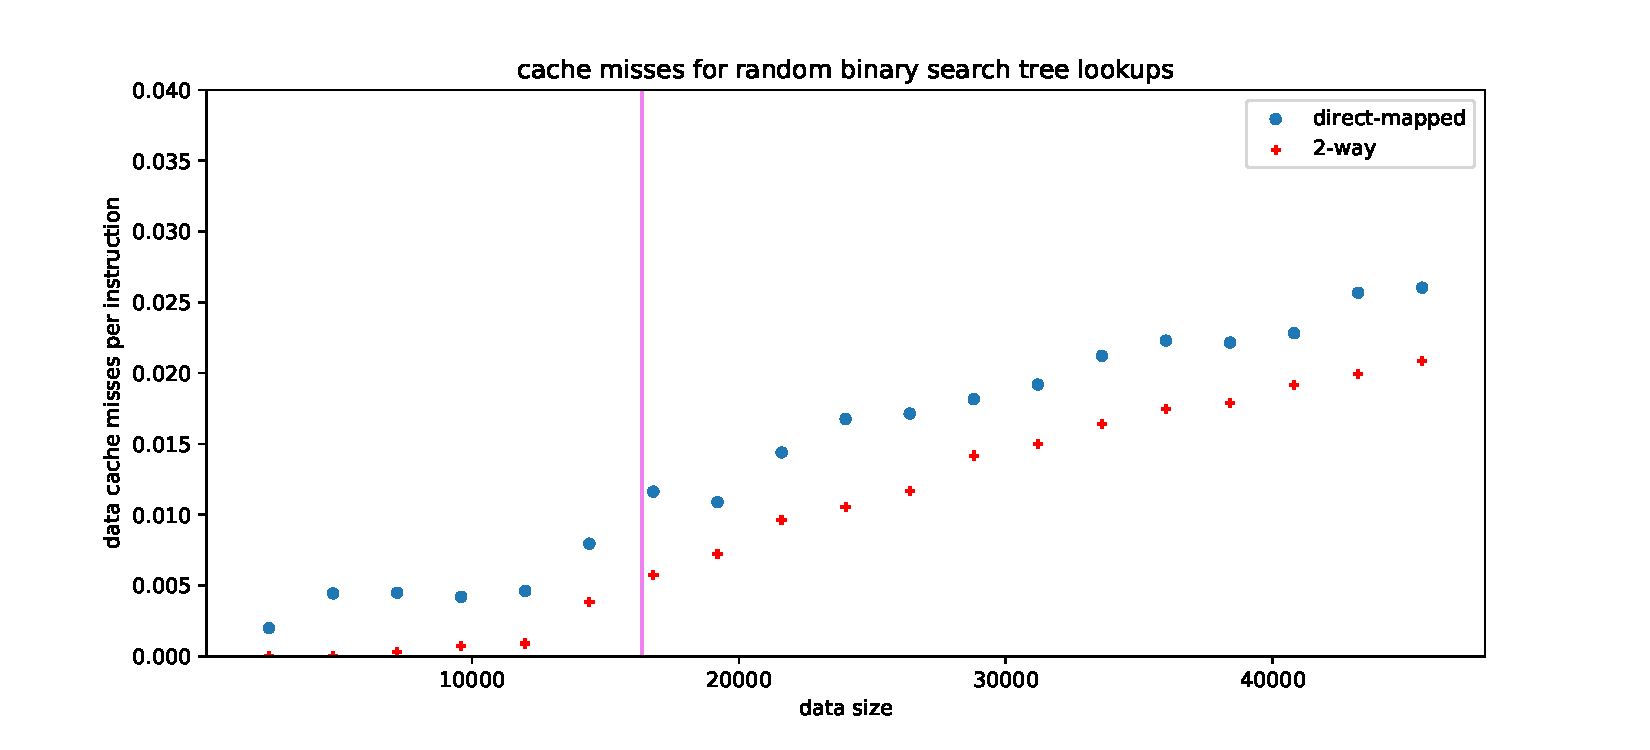
\includegraphics[width=\textwidth]{../caching/bst-both}
\end{frame}

\begin{frame}{actual misses: matrix multiplies}
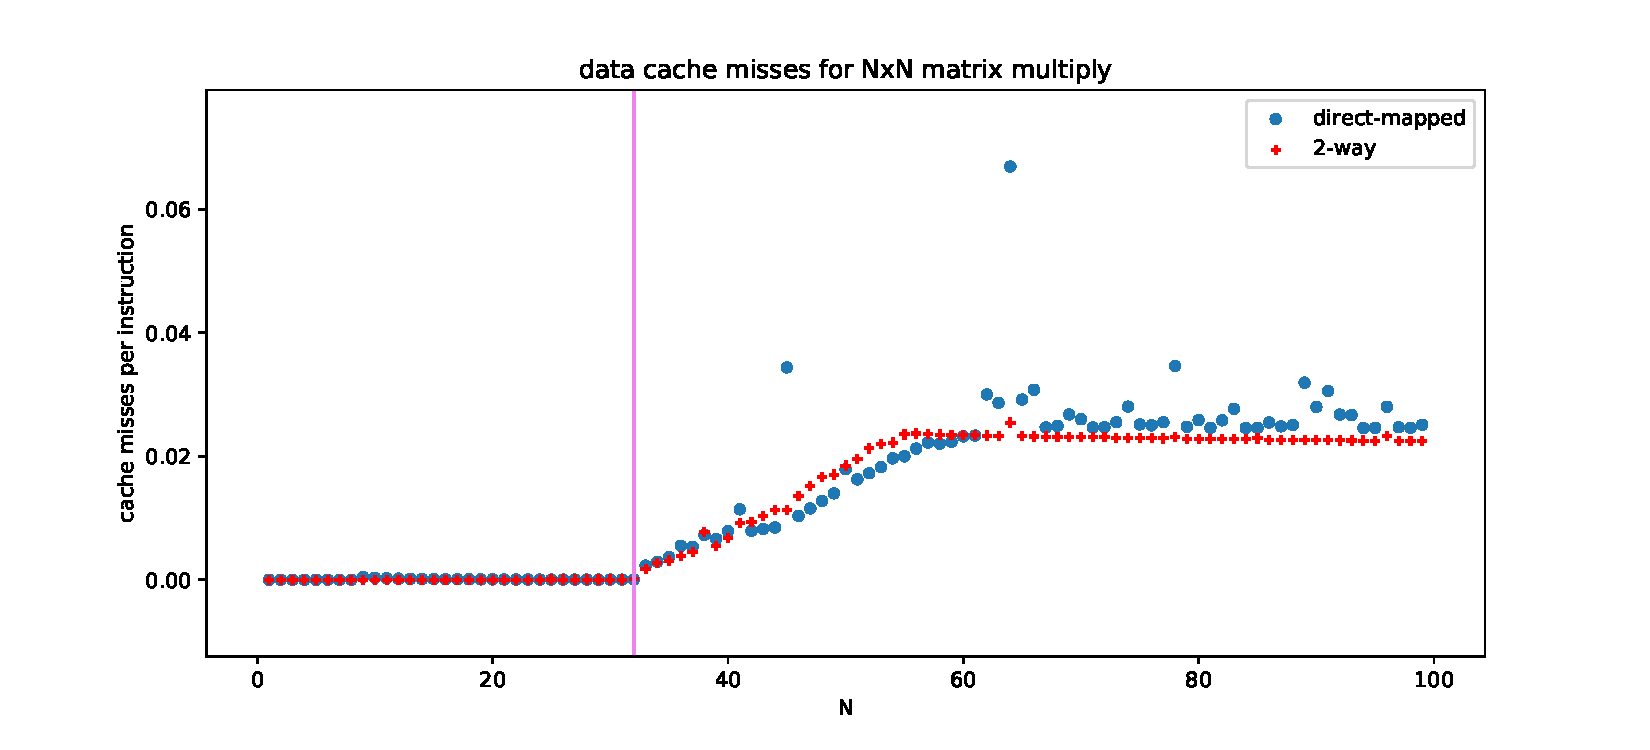
\includegraphics[width=\textwidth]{../caching/mm-both}
\end{frame}


\section{options for handling cache writes}
\usetikzlibrary{arrows.meta,matrix,positioning,shapes.callouts,shapes.misc,fit,calc}

\begin{frame}{handling writes}
    \begin{itemize}
    \item what about writing to the cache?
    \item two decision points:
    \vspace{.5cm}
    \item if the value is not in cache, do we add it?
        \begin{itemize}
        \item if yes: need to load rest of block
        \item if no: missing out on locality?
        \end{itemize}   
    \item if value is in cache, when do we update next level?
        \begin{itemize}
        \item if immediately: extra writing
        \item if later: need to remember to do so
        \end{itemize}
    \end{itemize}
\end{frame}

\begin{frame}{allocate on write?}
\begin{itemize}
\item processor writes \myemph{less than whole} cache block
\item block not yet in cache
\item two options:
\vspace{0.5cm}
\item \myemph{write-allocate}
    \begin{itemize}
    \item fetch rest of cache block, replace written part
    \item (then follow write-through or write-back policy)
    \end{itemize}
\item \myemph{write-no-allocate}
    \begin{itemize}
    \item don't use cache at all (send write to memory \textit{instead})
    \item guess: not read soon?
    \end{itemize}
\end{itemize}
\end{frame}

\begin{frame}{write-through v. write-back}
\begin{tikzpicture}
\tikzset{
    stepCircle/.style={circle,fill=yellow!10,draw,very thick,inner sep=1pt},
    every pin edge/.style={-,thick},
}

\node[draw,minimum width=1cm,minimum height=2.5cm] (cpu) {CPU};
\node[draw,minimum width=3cm,minimum height=4cm,right=4cm of cpu] (cache) {Cache};
    \node[above=2cm of cache,font=\bfseries] {
        \only<1-2>{option 1: write-through}\only<3-4>{option 2: write-back}
    };
\node[draw,minimum width=3cm,minimum height=6cm,right=4cm of cache] (mem) {RAM};
    \node[align=center,draw] (storedValue) at ([yshift=-1cm]cache.center) {{\tt ABCD}: \only<1>{FF}\only<2->{\myemph<2,3>{10}} \\ 
        \only<3->{(\myemph{dirty})}};
    \node[align=center,draw,anchor=north] (storedValueMem) at ([yshift=-.5cm]mem.center) {\ldots \\ {\tt 11CD}: {\tt 42} \\ {\tt ABCD}: \only<1,3>{FF}\only<2,4->{\myemph<4>{10}} \\ \ldots};

\begin{scope}[every node/.style={inner sep=1pt},every pin/.style={align=center}]
    \draw[very thick,-Latex] ([yshift=1cm]cpu.east) -- ([yshift=1cm]cache.west)
        node[-,midway,pin={[name=writeToCache]north:write {\tt 10}\\to {\tt 0xABCD}}] (cacheWrite) {};
    \node[stepCircle] at (writeToCache.north west) {1};
    \begin{visibleenv}<2>
        \draw[very thick,-Latex] ([yshift=1cm]cache.east) coordinate (cacheOut) --
            ([yshift=1cm]mem.west) coordinate (memIn)
            node[-,midway,pin={[name=forwardWrite]north:write {\tt 10}\\to {\tt 0xABCD}}] {};
        \node[stepCircle] at (forwardWrite.north west) {2};
    \end{visibleenv}
\end{scope}
\begin{visibleenv}<4->
    \node[draw,thick,cross out,minimum width=2cm,minimum height=1cm] at (storedValue) {};
\end{visibleenv}
\begin{visibleenv}<4->
    \node[pin={[align=center,name=readCmd]south:read \\ from \\ {\tt 0x11CD} \\ (conflicts)}] at (cacheWrite) {};
    \node[stepCircle] at (readCmd.north west) {2};
    \draw[very thick,-Latex] (cacheOut) -- (memIn)
        node[midway,pin={[align=center,name=writeBackOut]north:write {\tt 10} \\ to {\tt ABCD}}] {};
    \node[stepCircle] at (writeBackOut.north west) {3};
\end{visibleenv}
\begin{visibleenv}<4>
    \node[my callout2=storedValue.south,anchor=north] at ([yshift=-1cm]storedValue) {
        \ldots{} when replaced --- send value to memory
    };
\end{visibleenv}
\begin{visibleenv}<5->
    \path (cacheOut) -- (memIn)
        node[midway,pin={[align=center,name=actualRead]south:read\\from\\{\tt 0x11CD}}] {};
    \node[stepCircle] at (actualRead.north west) {4};
    \node[my callout2=actualRead.south,anchor=north] at ([xshift=1cm,yshift=-1cm]storedValue) {
        \ldots{} read new value to store in cache
    };
\end{visibleenv}
% FIXME: hilite hit miss in diagram, separate into animation
\end{tikzpicture}
\end{frame}

\begin{frame}[fragile,label=writebackBits]{writeback policy}
\begin{tikzpicture}
\tikzset{
    v/.style={visible on=<#1->,alt=<#1>{red}},
    h/.style={alt=<#1>{red}},
    tagColor/.style={color=green!60!black},
    dataColor/.style={color=blue!60!black},
    offsetColor/.style={color=yellow!30!black},
}
\matrix[tight matrix,
        nodes={font=\small\tt,text depth=.1ex,text height=1ex,minimum height=1cm},
        row 1/.append style={nodes={font=\small\bfseries,minimum height=.5cm}},
        column 1/.append style={nodes={draw=none,text width=1.2cm,align=center}},
        column 2/.append style={nodes={align=center,text width=1cm}},
        column 3/.append style={nodes={align=center,tagColor,text width=1.7cm,
            font=\tt\fontsize{10}{11}\selectfont}},
        column 4/.append style={nodes={text width=1.5cm,align=center,dataColor,
            text depth=2.3ex,font=\tt\fontsize{7}{8}\selectfont}},
        column 5/.append style={nodes={align=center,text width=1cm,red}},
        column 6/.append style={nodes={draw=none,text width=.1cm}},
        column 7/.append style={nodes={align=center,text width=0.9cm}},
        column 8/.append style={nodes={align=center,tagColor,text width=1.7cm,
            font=\tt\fontsize{10}{11}\selectfont}},
        column 9/.append style={nodes={text width=1.5cm,align=center,dataColor,
            text depth=2.3ex,font=\tt\fontsize{7}{8}\selectfont}},
        column 10/.append style={nodes={align=center,text width=1cm,red}},
        column 11/.append style={nodes={draw=none,text width=.1cm}},
        column 12/.append style={nodes={align=center}},
        row 1 column 4/.append style={nodes={text depth=.1ex,font=\small\bfseries}},
        row 1 column 9/.append style={nodes={text depth=.1ex,font=\small\bfseries}},
        row 1 column 10/.append style={nodes={align=center,text width=1cm}},
        label={[font=\small]$2$-way set associative, $4$ byte blocks, $2$ sets}] (cache)  {
index \& valid \& tag \& value \& dirty \& ~\& valid \& tag \& value \& dirty \& ~\&LRU \\
0\&
    % i 0, 0:
    1 \& 
    000000 \& 
    mem[0x00] mem[0x01] \&
    0 \& ~\&
    % i 0, 1:
    1 \& 
    011000 \& 
    mem[0x60]* mem[0x61]* \&
    1 \& ~ \&
    1 \\
1\& 
    % i 1, 0:
    1 \& 
    011000 \&
    mem[0x62] mem[0x63] \& 
    0 \& ~\&
    % i 1, 1:
    0 \& ~ \& ~ \&  ~ \&
    ~ \& 0
    \\
};

\node[my callout2=cache-2-9.north,anchor=south,align=left] at ([yshift=2cm,xshift=-4cm]cache-2-9.north) {
    changed value!
};
\node[my callout2=cache-2-10.south,anchor=north,align=left] at ([yshift=-1cm,xshift=-4cm]cache-2-10.south) {
    1 = dirty (different than memory) \\ needs to be written if evicted
};
\end{tikzpicture}
\end{frame}

\begin{frame}[fragile,label=writeAllocateEx]{write-allocate + write-back}
\begin{tikzpicture}
\tikzset{
    v/.style={visible on=<#1->,alt=<#1>{red}},
    h/.style={alt=<#1>{red}},
    tagColor/.style={color=green!60!black},
    dataColor/.style={color=blue!60!black},
    offsetColor/.style={color=yellow!30!black},
}
\matrix[tight matrix,
        nodes={font=\small\tt,text depth=.1ex,text height=1ex,minimum height=1cm},
        row 1/.append style={nodes={font=\small\bfseries,minimum height=.5cm}},
        column 1/.append style={nodes={draw=none,text width=1.2cm,align=center}},
        column 2/.append style={nodes={align=center,text width=1cm}},
        column 3/.append style={nodes={align=center,tagColor,text width=1.7cm,
            font=\tt\fontsize{10}{11}\selectfont}},
        column 4/.append style={nodes={text width=1.3cm,align=center,dataColor,
            text depth=2.3ex,font=\tt\fontsize{7}{8}\selectfont}},
        column 5/.append style={nodes={align=center,text width=1cm,red}},
        column 6/.append style={nodes={draw=none,text width=.1cm}},
        column 7/.append style={nodes={align=center,text width=0.9cm}},
        column 8/.append style={nodes={align=center,tagColor,text width=1.7cm,
            font=\tt\fontsize{10}{11}\selectfont}},
        column 9/.append style={nodes={text width=1.3cm,align=center,dataColor,
            text depth=2.3ex,font=\tt\fontsize{7}{8}\selectfont}},
        column 10/.append style={nodes={align=center,text width=1cm,red}},
        column 11/.append style={nodes={draw=none,text width=.1cm}},
        column 12/.append style={nodes={align=center}},
        row 1 column 4/.append style={nodes={text depth=.1ex,font=\small\bfseries}},
        row 1 column 9/.append style={nodes={text depth=.1ex,font=\small\bfseries}},
        row 1 column 10/.append style={nodes={align=center,text width=1cm}},
        label={[font=\small]$2$-way set associative, LRU, writeback}] (cache)  {
index \& valid \& tag \& value \& dirty \& ~\& valid \& tag \& value \& dirty \& ~\&LRU \\
0\&
    % i 0, 0:
    1 \& 
    000000 \& 
    mem[0x00] mem[0x01] \&
    0 \& ~\&
    % i 0, 1:
    1 \& 
    \only<1-3>{011000}\only<4->{000001} \& 
    \only<1-3>{mem[0x60]* mem[0x61]*}%
    \only<4->{0xFF mem[0x05]}%
     \&
    \sout<3>{1} \& ~ \&
    |[h=2]| \only<1-3>{1}\only<4->{\myemph<4>{0}} \\
1\& 
    % i 1, 0:
    1 \& 
    011000 \&
    mem[0x62] mem[0x63] \& 
    0 \& ~\&
    % i 1, 1:
    0 \& ~ \& ~ \&  ~ \&
    ~ \& 0
    \\
};
\begin{visibleenv}<2-3>
    \node[inner sep=-1pt,line width=2pt,red,draw,fit=(cache-2-7) (cache-2-10)] {};
\end{visibleenv}
\node[anchor=north west,align=left] at ([yshift=-.1cm]cache.south west) {
    \myemph{writing} {\t 0xFF} into address {\tt 0x04}? \\
    index 0, tag 000001 \\
    \only<2->{step 1: find \myemph{least recently used} block} \\
    \only<3->{step 2: possibly writeback old block} \\
    \only<4->{step 3a: read in new block -- to get mem[0x05]} \\
    \only<4->{step 3b: update LRU information}
};
\end{tikzpicture}
\end{frame}

\begin{frame}[fragile,label=writeNoAllocateEx]{write-no-allocate + write-back}
\begin{tikzpicture}
\tikzset{
    v/.style={visible on=<#1->,alt=<#1>{red}},
    h/.style={alt=<#1>{red}},
    tagColor/.style={color=green!60!black},
    dataColor/.style={color=blue!60!black},
    offsetColor/.style={color=yellow!30!black},
}
\matrix[tight matrix,
        nodes={font=\small\tt,text depth=.1ex,text height=1ex,minimum height=1cm},
        row 1/.append style={nodes={font=\small\bfseries,minimum height=.5cm}},
        column 1/.append style={nodes={draw=none,text width=1.2cm,align=center}},
        column 2/.append style={nodes={align=center,text width=1cm}},
        column 3/.append style={nodes={align=center,tagColor,text width=1.3cm,
            font=\tt\fontsize{10}{11}\selectfont}},
        column 4/.append style={nodes={text width=1.3cm,align=center,dataColor,
            text depth=2.3ex,font=\tt\fontsize{7}{8}\selectfont}},
        column 5/.append style={nodes={align=center,text width=1cm,red}},
        column 6/.append style={nodes={draw=none,text width=.1cm}},
        column 7/.append style={nodes={align=center,text width=0.9cm}},
        column 8/.append style={nodes={align=center,tagColor,text width=1.3cm,
            font=\tt\fontsize{10}{11}\selectfont}},
        column 9/.append style={nodes={text width=1.3cm,align=center,dataColor,
            text depth=2.3ex,font=\tt\fontsize{7}{8}\selectfont}},
        column 10/.append style={nodes={align=center,text width=1cm,red}},
        column 11/.append style={nodes={draw=none,text width=.1cm}},
        column 12/.append style={nodes={align=center}},
        row 1 column 4/.append style={nodes={text depth=.1ex,font=\small\bfseries}},
        row 1 column 9/.append style={nodes={text depth=.1ex,font=\small\bfseries}},
        row 1 column 10/.append style={nodes={align=center,text width=1cm}},
        label={[font=\small]$2$-way set associative, LRU, writeback}] (cache)  {
index \& valid \& tag \& value \& dirty \& ~\& valid \& tag \& value \& dirty \& ~\&LRU \\
0\&
    % i 0, 0:
    1 \& 
    000000 \& 
    mem[0x00] mem[0x01] \&
    0 \& ~\&
    % i 0, 1:
    1 \& 
    011000 \& 
    mem[0x60]* mem[0x61]*%
    %
     \&
    1 \& ~ \&
    1 \\
1\& 
    % i 1, 0:
    1 \& 
    011000 \&
    mem[0x62] mem[0x63] \& 
    0 \& ~\&
    % i 1, 1:
    0 \& ~ \& ~ \&  ~ \&
    ~ \& 0
    \\
};
\begin{visibleenv}<1>
    \node[inner sep=-1pt,line width=2pt,red,draw,fit=(cache-2-7) (cache-2-10)] {};
\end{visibleenv}
\node[anchor=north west,align=left] at ([yshift=-.1cm]cache.south west) {
    \myemph{writing} {\t 0xFF} into address {\tt 0x04}? \\
    step 1: is it in cache yet? \\
    step 2: no, \myemph{just send it to memory}
};
\end{tikzpicture}
\end{frame}




\subsection{exercise: write/replacement policies}
\usetikzlibrary{fit,matrix}
\begin{frame}[fragile,label=writeReplaceEx1]{exercise (1)}
\begin{tikzpicture}
\tikzset{
    v/.style={visible on=<#1->,alt=<#1>{red}},
    h/.style={alt=<#1>{red}},
    tagColor/.style={color=green!60!black},
    dataColor/.style={color=blue!60!black},
    offsetColor/.style={color=yellow!30!black},
}
\matrix[tight matrix,
        nodes={font=\small\tt,text depth=.1ex,text height=1ex,minimum height=1cm},
        row 1/.append style={nodes={font=\small\bfseries,minimum height=.5cm}},
        column 1/.append style={nodes={draw=none,text width=1.2cm,align=center}},
        column 2/.append style={nodes={align=center,text width=1cm}},
        column 3/.append style={nodes={align=center,tagColor,text width=1.3cm,
            font=\tt\fontsize{10}{11}\selectfont}},
        column 4/.append style={nodes={text width=1.3cm,align=center,dataColor,
            text depth=2.3ex,font=\tt\fontsize{7}{8}\selectfont}},
        column 5/.append style={nodes={align=center,text width=1cm,red}},
        column 6/.append style={nodes={draw=none,text width=.1cm}},
        column 7/.append style={nodes={align=center,text width=0.9cm}},
        column 8/.append style={nodes={align=center,tagColor,text width=1.3cm,
            font=\tt\fontsize{10}{11}\selectfont}},
        column 9/.append style={nodes={text width=1.3cm,align=center,dataColor,
            text depth=2.3ex,font=\tt\fontsize{7}{8}\selectfont}},
        column 10/.append style={nodes={align=center,text width=1cm,red}},
        column 11/.append style={nodes={draw=none,text width=.1cm}},
        column 12/.append style={nodes={align=center}},
        row 1 column 4/.append style={nodes={text depth=.1ex,font=\small\bfseries}},
        row 1 column 9/.append style={nodes={text depth=.1ex,font=\small\bfseries}},
        row 1 column 10/.append style={nodes={align=center,text width=1cm}},
        label={[font=\small]$2$-way set associative, LRU, \myemph{write-allocate, writeback}}] (cache)  {
index \& valid \& tag \& value \& dirty \& ~\& valid \& tag \& value \& dirty \& ~\&LRU \\
0\&
    % i 0, 0:
    1 \& 
    001100 \& 
    mem[0x30] mem[0x31] \&
    0 \& ~\&
    % i 0, 1:
    1 \& 
    010000 \& 
    mem[0x40]* mem[0x41]*%
    %
     \&
    1 \& ~ \&
    0 \\
1 \& 
    % i 1, 0:
    1 \& 
    011000 \&
    mem[0x62] mem[0x63] \& 
    0 \& ~ \&
    1 \&  
    001100 \&
    % i 1, 1:
    mem[0x32]* mem[0x33]* \& 1 \&  ~ \&
    1
    \\
};
\end{tikzpicture}
\begin{itemize}
\item
for each of the following accesses, performed alone, would it require (a) reading a value from memory (or next level of cache) and (b) writing a value to the memory (or next level of cache)?
    \begin{itemize}
    \item writing 1 byte to 0x33
    \item reading 1 byte from 0x52
    \item reading 1 byte from 0x50
    \end{itemize}
\end{itemize}
\end{frame}


\begin{frame}<0>[fragile,label=writeReplaceEx1Soln]{exercise (1, solution)}
\begin{tikzpicture}
\tikzset{
    v/.style={visible on=<#1->,alt=<#1>{red}},
    h/.style={alt=<#1>{red}},
    tagColor/.style={color=green!60!black},
    dataColor/.style={color=blue!60!black},
    offsetColor/.style={color=yellow!30!black},
}
\matrix[tight matrix,
        nodes={font=\small\tt,text depth=.1ex,text height=1ex,minimum height=1cm},
        row 1/.append style={nodes={font=\small\bfseries,minimum height=.5cm}},
        column 1/.append style={nodes={draw=none,text width=1.2cm,align=center}},
        column 2/.append style={nodes={align=center,text width=1cm}},
        column 3/.append style={nodes={align=center,tagColor,text width=1.3cm,
            font=\tt\fontsize{10}{11}\selectfont}},
        column 4/.append style={nodes={text width=1.3cm,align=center,dataColor,
            text depth=2.3ex,font=\tt\fontsize{7}{8}\selectfont}},
        column 5/.append style={nodes={align=center,text width=1cm,red}},
        column 6/.append style={nodes={draw=none,text width=.1cm}},
        column 7/.append style={nodes={align=center,text width=0.9cm}},
        column 8/.append style={nodes={align=center,tagColor,text width=1.3cm,
            font=\tt\fontsize{10}{11}\selectfont}},
        column 9/.append style={nodes={text width=1.6cm,align=center,dataColor,
            text depth=2.3ex,font=\tt\fontsize{7}{8}\selectfont}},
        column 10/.append style={nodes={align=center,text width=1cm,red}},
        column 11/.append style={nodes={draw=none,text width=.1cm}},
        column 12/.append style={nodes={align=center}},
        row 1 column 4/.append style={nodes={text depth=.1ex,font=\small\bfseries}},
        row 1 column 9/.append style={nodes={text depth=.1ex,font=\small\bfseries}},
        row 1 column 10/.append style={nodes={align=center,text width=1cm}},
        label={[font=\small]$2$-way set associative, LRU, \myemph{write-allocate, writeback}}] (cache)  {
index \& valid \& tag \& value \& dirty \& ~\& valid \& tag \& value \& dirty \& ~\&LRU \\
0\&
    % i 0, 0:
    1 \& 
    |[alias=problem3tag]| 001100 \& 
    |[alias=problem3data]| mem[0x30] mem[0x31] \&
    0 \& ~\&
    % i 0, 1:
    1 \& 
    010000 \& 
     mem[0x40]* mem[0x41]*%
    %
     \&
    1 \& ~ \&
    |[alias=problem3lru]| 0 \\
1 \& 
    % i 1, 0:
    1 \& 
    011000 \&
    mem[0x62] mem[0x63] \& 
    0 \& ~ \&
    1 \&  
    |[alias=problem1tag,alias=problem2tag]| 001100 \&
    % i 1, 1:
    |[alias=problem1data,alias=problem2data]| {mem[0x32]* mem[0x33]*} \& |[alias=problem1dirty,alias=problem2dirty]| {1} \&  ~ \&
    |[alias=problem1lru,alias=problem2lru]|1
    \\
};
    \begin{visibleenv}<2>
        \node[fit=(problem1data),inner sep=0mm,draw=red,ultra thick,fill=red,fill opacity=0.10] {};
        \node[fit=(problem1lru),inner sep=0mm,draw=red,ultra thick,fill=red!10,text=red] {\sout{1}0};
    \end{visibleenv}
    \begin{visibleenv}<4>
        \node[fit=(problem2data),inner sep=0mm,draw=red,ultra thick,fill=red!10,text=red,
              font=\tt\fontsize{7}{8}\selectfont] {
                mem[0x52]\\mem[0x53]
            };
        \node[fit=(problem2dirty),inner sep=0mm,draw=red,ultra thick,fill=red!10,text=red] {\sout{1}0};
        \node[fit=(problem2lru),inner sep=0mm,draw=red,ultra thick,fill=red!10,text=red] {\sout{1}0};
        \node[fit=(problem2tag),inner sep=0mm,draw=red,ultra thick,fill=red!10,text=red,font=\tt\fontsize{10}{11}\selectfont] {101000};
    \end{visibleenv}
    \begin{visibleenv}<6>
        \node[fit=(problem3data),inner sep=0mm,draw=red,ultra thick,fill=red!10,text=red,
              font=\tt\fontsize{7}{8}\selectfont] {
                mem[0x50]\\mem[0x51]
            };
        \node[fit=(problem3lru),inner sep=0mm,draw=red,ultra thick,fill=red!10,text=red] {\sout{0}1};
        \node[fit=(problem3tag),inner sep=0mm,draw=red,ultra thick,fill=red!10,text=red,font=\tt\fontsize{10}{11}\selectfont] {101000};
    \end{visibleenv}
\end{tikzpicture}
\begin{itemize}
\item \myemph<1-2>{writing 1 byte to 0x33}: \only<1->{(set 1, offset 1) no read or write}
\item \myemph<3-4>{reading 1 byte from 0x52}: \only<3->{(set 1, offset 0) \textbf{write} back 0x32-0x33; \textbf{read} 0x52-0x53}
\item \myemph<5-6>{reading 1 byte from 0x50}: \only<5->{(set 0, offset 0) replace 0x30-0x31 (no write back); \textbf{read} 0x50-0x51}
\end{itemize}
\end{frame}

\iftoggle{heldback}{}{
    \againframe<1->{writeReplaceEx1Soln}
}

\begin{frame}[fragile,label=writeReplaceEx2]{exercise (2)}
\begin{tikzpicture}
\tikzset{
    v/.style={visible on=<#1->,alt=<#1>{red}},
    h/.style={alt=<#1>{red}},
    tagColor/.style={color=green!60!black},
    dataColor/.style={color=blue!60!black},
    offsetColor/.style={color=yellow!30!black},
}
\matrix[tight matrix,
        nodes={font=\small\tt,text depth=.1ex,text height=1ex,minimum height=1cm},
        row 1/.append style={nodes={font=\small\bfseries,minimum height=.5cm}},
        column 1/.append style={nodes={draw=none,text width=1.2cm,align=center}},
        column 2/.append style={nodes={align=center,text width=1cm}},
        column 3/.append style={nodes={align=center,tagColor,text width=1.3cm,
            font=\tt\fontsize{10}{11}\selectfont}},
        column 4/.append style={nodes={text width=1.3cm,align=center,dataColor,
            text depth=2.3ex,font=\tt\fontsize{7}{8}\selectfont}},
        column 5/.append style={nodes={align=center,text width=1cm,red}},
        column 6/.append style={nodes={draw=none,text width=.1cm}},
        column 7/.append style={nodes={align=center,text width=0.9cm}},
        column 8/.append style={nodes={align=center,tagColor,text width=1.3cm,
            font=\tt\fontsize{10}{11}\selectfont}},
        column 9/.append style={nodes={text width=1.3cm,align=center,dataColor,
            text depth=2.3ex,font=\tt\fontsize{7}{8}\selectfont}},
        column 10/.append style={nodes={align=center,text width=1cm,red}},
        column 11/.append style={nodes={draw=none,text width=.1cm}},
        column 12/.append style={nodes={align=center}},
        row 1 column 4/.append style={nodes={text depth=.1ex,font=\small\bfseries}},
        row 1 column 9/.append style={nodes={text depth=.1ex,font=\small\bfseries}},
        row 1 column 10/.append style={nodes={align=center,text width=1cm}},
        label={[font=\small]$2$-way set associative, LRU, \myemph{write-no-allocate, write-through}}] (cache)  {
index \& valid \& tag \& value \& \& ~\& valid \& tag \& value \& \& ~\&LRU \\
0\&
    % i 0, 0:
    1 \& 
    001100 \& 
    mem[0x30] mem[0x31] \&
     \& ~\&
    % i 0, 1:
    1 \& 
    010000 \& 
    mem[0x40] mem[0x41]%
    %
     \&
    \& ~ \&
    0 \\
1 \& 
    % i 1, 0:
    1 \& 
    011000 \&
    mem[0x62] mem[0x63] \& 
     \& ~ \&
    1 \&  
    001100 \&
    % i 1, 1:
    mem[0x32] mem[0x33] \&  \&  ~ \&
    1
    \\
};
\end{tikzpicture}
\begin{itemize}
\item
for each of the following accesses, performed alone, would it require (a) reading a value from memory and (b) writing a value to the memory?
    \begin{itemize}
    \item writing 1 byte to 0x33
    \item reading 1 byte from 0x52
    \item reading 1 byte from 0x50
    
    \end{itemize}
\end{itemize}
\end{frame}

\begin{frame}<0>[fragile,label=writeReplaceEx2Soln]{exercise (2, solution)}
\begin{tikzpicture}
\tikzset{
    v/.style={visible on=<#1->,alt=<#1>{red}},
    h/.style={alt=<#1>{red}},
    tagColor/.style={color=green!60!black},
    dataColor/.style={color=blue!60!black},
    offsetColzAor/.style={color=yellow!30!black},
}
\matrix[tight matrix,
        nodes={font=\small\tt,text depth=.1ex,text height=1ex,minimum height=1cm},
        row 1/.append style={nodes={font=\small\bfseries,minimum height=.5cm}},
        column 1/.append style={nodes={draw=none,text width=1.2cm,align=center}},
        column 2/.append style={nodes={align=center,text width=1cm}},
        column 3/.append style={nodes={align=center,tagColor,text width=1.3cm,
            font=\tt\fontsize{10}{11}\selectfont}},
        column 4/.append style={nodes={text width=1.3cm,align=center,dataColor,
            text depth=2.3ex,font=\tt\fontsize{7}{8}\selectfont}},
        column 5/.append style={nodes={align=center,text width=1cm,red}},
        column 6/.append style={nodes={draw=none,text width=.1cm}},
        column 7/.append style={nodes={align=center,text width=0.9cm}},
        column 8/.append style={nodes={align=center,tagColor,text width=1.3cm,
            font=\tt\fontsize{10}{11}\selectfont}},
        column 9/.append style={nodes={text width=1.3cm,align=center,dataColor,
            text depth=2.3ex,font=\tt\fontsize{7}{8}\selectfont}},
        column 10/.append style={nodes={align=center,text width=1cm,red}},
        column 11/.append style={nodes={draw=none,text width=.1cm}},
        column 12/.append style={nodes={align=center}},
        row 1 column 4/.append style={nodes={text depth=.1ex,font=\small\bfseries}},
        row 1 column 9/.append style={nodes={text depth=.1ex,font=\small\bfseries}},
        row 1 column 10/.append style={nodes={align=center,text width=1cm}},
        label={[font=\small]$2$-way set associative, LRU, \myemph{write-no-allocate, write-through}}] (cache)  {
index \& valid \& tag \& value \& \& ~\& valid \& tag \& value \& \& ~\&LRU \\
0\&
    % i 0, 0:
    1 \& 
    |[alias=problem3tag]| 001100 \& 
    |[alias=problem3data]| mem[0x30] mem[0x31] \&
     \& ~\&
    % i 0, 1:
    1 \& 
    010000 \& 
    mem[0x40] mem[0x41]%
    %
     \&
    \& ~ \&
    |[alias=problem3lru]| 0 \\
1 \& 
    % i 1, 0:
    1 \& 
    011000 \&
    mem[0x62] mem[0x63] \& 
     \& ~ \&
    1 \&  
    |[alias=problem1tag,alias=problem2tag]|001100 \&
    % i 1, 1:
    |[alias=problem1data,alias=problem2data]| {mem[0x32] mem[0x33]} \& \&  ~ \&
    |[alias=problem1lru,alias=problem2lru]| 1
    \\
};
    \begin{visibleenv}<2>
        \node[fit=(problem1data),inner sep=0mm,draw=red,ultra thick,fill=red,fill opacity=0.10] {};
        \node[fit=(problem1lru),inner sep=0mm,draw=red,ultra thick,fill=red!10,text=red] {\sout{1}0};
    \end{visibleenv}
    \begin{visibleenv}<4>
        \node[fit=(problem2data),inner sep=0mm,draw=red,ultra thick,fill=red!10,text=red,
              font=\tt\fontsize{7}{8}\selectfont] {
                mem[0x52]\\mem[0x53]
            };
        \node[fit=(problem2lru),inner sep=0mm,draw=red,ultra thick,fill=red!10,text=red] {\sout{1}0};
        \node[fit=(problem2tag),inner sep=0mm,draw=red,ultra thick,fill=red!10,text=red,font=\tt\fontsize{10}{11}\selectfont] {101000};
    \end{visibleenv}
    \begin{visibleenv}<6>
        \node[fit=(problem3data),inner sep=0mm,draw=red,ultra thick,fill=red!10,text=red,
              font=\tt\fontsize{7}{8}\selectfont] {
                mem[0x50]\\mem[0x51]
            };
        \node[fit=(problem3lru),inner sep=0mm,draw=red,ultra thick,fill=red!10,text=red] {\sout{0}1};
        \node[fit=(problem3tag),inner sep=0mm,draw=red,ultra thick,fill=red!10,text=red,font=\tt\fontsize{10}{11}\selectfont] {101000};
    \end{visibleenv}
\end{tikzpicture}
\begin{itemize}
\item \myemph<1-2>{writing 1 byte to 0x33}: \only<1->{(set 1, offset 1) write-through 0x33 modification}
\item \myemph<3-4>{reading 1 byte from 0x52}: \only<3->{(set 1, offset 0) replace 0x32-0x33; \textbf{read} 0x52-0x53}
\item \myemph<5-6>{reading 1 byte from 0x50}: \only<5->{(set 0, offset 0) replace 0x30-0x31; \textbf{read} 0x50-0x51}
\end{itemize}
\end{frame}

\iftoggle{heldback}{}{
    \againframe<1->{writeReplaceEx2Soln}
}


\subsection{fast writes: write buffers}
\usetikzlibrary{arrows.meta,positioning}

\begin{frame}{fast writes}
\begin{tikzpicture}
    \tikzset{every pin edge/.style={-,thick}}
\node[draw,minimum width=1cm,minimum height=2.5cm] (cpu) {CPU};
\node[draw,minimum width=3cm,minimum height=4cm,right=3cm of cpu] (cache) {Cache};
\node[draw,minimum width=1cm,minimum height=6cm,right=3cm of cache] (mem) {RAM};
\draw[very thick,-Latex] ([yshift=1cm]cpu.east) -- ([yshift=1cm]cache.west)
    node[-,midway,pin={[align=center,-]north:write {\tt 10}\\to {\tt 0xABCD}}] (cacheWrite) {};
\draw[very thick,-Latex] ([yshift=1cm]cpu.east) -- ([yshift=1cm]cache.west)
    node[-,midway,pin={[align=center,-]south:write {\tt 20}\\to {\tt 0x1234}}] (cacheWrite2) {};
\draw[very thick,dashed,-Latex] ([yshift=1cm]cache.east) coordinate (cacheOut) --
    ([yshift=1cm]mem.west) coordinate (memIn)
    node[align=left,font=\tt,red,very thick,near start,label={[font=\bfseries]write buffer},draw,fill=white] { 0xABCD: 10 \\ 0x1234: 20 };

    \node[draw=red,fill=white,below=.5cm of cache,align=left] {%
         write appears to complete immediately when placed in buffer \\
         buffer checked on reads in case reading just-evicted value
    };
\end{tikzpicture}
\end{frame}


\subsection{briefly, cache tradeoffs}
\begin{frame}{cache tradeoffs briefly}
    \begin{itemize}
    \item deciding cache size, associativity, etc.?
    \item lots of tradeoffs:
        \begin{itemize}
        \item more cache hits v. slower cache hits?
        \item faster cache hits v. fewer cache hits?
        \item (N+1)th-level cache v. larger Nth level cache?
        \item \ldots
        \end{itemize}
    \item details depend on programs run
        \begin{itemize}
        \item how often is same block used again?
        \item how often is same index bits used?
        \item how much \{temporal,spatial\} locality to take advantage of?
        \end{itemize}
    \item simulation to assess impact of designs
    \end{itemize}
\end{frame}


\section{TLB}
\usetikzlibrary{arrows.meta, fit}
\begin{frame}<0>[label=twoLevelPtLookup]{two-level page table lookup}
\begin{tikzpicture}
\tikzset{
    >=Latex,
    pageNumber/.style={fill=blue!10,font=\fontsize{11}{12}\selectfont,inner sep=.5mm},
    pageNumberA/.style={fill=violet!30,font=\fontsize{11}{12}\selectfont,inner sep=.5mm,draw,thick,dotted},
    pageNumberB/.style={fill=brown!20,font=\fontsize{11}{12}\selectfont,inner sep=.5mm,draw,thick,dotted},
    pageOffset/.style={fill=green!20,font=\fontsize{11}{12}\selectfont,inner sep=.5mm},
    comp/.style={fill=yellow!10,font=\fontsize{11}{12}\selectfont,draw},
    memAccess/.style={alt=<all:7>{red, very thick}},
    pageNumberExpand/.style={alt=<all:11>{draw=red,very thick}},
    smallLabel/.style={fill=white,draw,thick,font=\fontsize{10}{11}\selectfont,inner sep=.5mm,align=center},
}
\node[pageNumberA] (addrLeftA) {11 0101 01};
\node[pageNumberB,anchor=west] (addrLeftB) at (addrLeftA.east) {00 1011 00};
\node[anchor=west,pageOffset] (addrRight) at (addrLeftB.east) {00 1101 1111};
\node[inner sep=0mm,draw=none,fit=(addrLeftA) (addrLeftB),alt=<1>{draw=red,very thick}] (addrLeft) {};
\begin{visibleenv}<all:1>
\node[below=1cm of addrLeft,xshift=2cm] (vpn split explain) {VPN --- split into two parts (one per level)};
\node[below=1cm of vpn split explain,font=\small] {
    this example: parts equal sized --- common, but not required
};
\end{visibleenv}
\begin{visibleenv}<all:2->
\node[draw,comp,below=1cm of addrLeftA,align=center,xshift=-1cm] (timesPte) {$\times$ \\ PTE \\ size};
\draw[->,thick] (addrLeftA) -- ++(0cm,-.5cm) -| (timesPte);
\node[font=\tt\fontsize{10}{11}\selectfont,draw,very thick,left=0.25cm of addrLeft,label={[align=center,font=\small]north:page table\\base register},yshift=-.5cm] (ptbr) {0x10000};
\node[draw,comp] (plus) at ([yshift=-1cm]timesPte.south) {+};
\draw[->,thick] (timesPte) -- (plus);
\draw[->,thick] (ptbr) |- (plus);
\end{visibleenv}

\begin{visibleenv}<all:3->
\node[below=1.5cm of plus,fill=violet!10,draw,very thick,minimum height=1cm,minimum width=15cm,xshift=5.5cm] (cache) {memory {\small (really cache)}};
\end{visibleenv}
\begin{visibleenv}<all:5->
\node[pageNumber] (addrLeftFinal) at ([xshift=9.6cm,yshift=-1cm]plus) {1101 0011 11};
\end{visibleenv}
\begin{visibleenv}<all:3->
\draw[->,thick,memAccess] (plus) -- (cache.north -| plus.south) node[midway,smallLabel] {1st PTE \\ addr.};
\node[above right=1cm and .5cm of plus,align=center,draw,comp,font=\small] (check) {valid, etc?};
\node[below=.75cm of check,draw,comp,align=center] (splitA) {split  \\ PTE parts};
\draw[->,thick] (cache.north -| splitA.south) -- (splitA.south);
\draw[->,thick] (splitA) -- (check);
\draw[->,thick] (check.north) -- ++(0,.75cm) node[above,font=\small,inner sep=.5mm] {cause fault?};
\end{visibleenv}

\begin{visibleenv}<all:4->
    \node[comp,align=center,right=.75cm of splitA,pageNumberExpand] (timesSize){$\times$ \\ page \\ size};
    \node[comp,align=center,right=1.25cm of timesSize] (plusB) {+};
    \draw[brown!60!black,->,thick,pageNumberExpand] (splitA) -- (timesSize);
    \draw[dotted,black,thick] ($(splitA.east)!0.5!(timesSize.west)$) -- ++ (0cm, .5cm) node[above,font=\fontsize{10}{11}\selectfont,align=center] {phys\\page \#};
    \draw[brown!60!black,->,thick,pageNumberExpand] (timesSize) -- (plusB);
    \draw[dotted,black,thick] ($(plusB.east)!0.5!(timesSize.west)$) -- ++ (0cm, .5cm) node[above,font=\fontsize{10}{11}\selectfont,align=center] {phys\\addr};
    \draw[memAccess,->,thick] (plusB) -- (plusB |- cache.north) node[midway,smallLabel]{2nd PTE \\ addr.};
    \node[comp,align=center,above=.5cm of plusB] (timesPteB) {$\times$ \\ PTE \\ size};
    \draw[brown!60!black,->,thick] (addrLeftB) -- ++(0cm,-.5cm) -| (timesPteB.north);
    \draw[brown!60!black,->,thick] (timesPteB) -- (plusB);
\end{visibleenv}

\begin{visibleenv}<all:5->
\node[right=.5cm of plusB,draw,comp,align=center] (splitB) {split  \\ PTE parts};
\draw[->,thick] (cache.north -| splitB.south) -- (splitB.south);
\node[above=.75cm of splitB,align=center,draw,comp,font=\small] (checkB) {valid, etc?};
\draw[->,thick] (splitB) -- (checkB);
\draw[->,thick] (checkB.north) -- ++(0cm, .75cm) node[above,font=\small,inner sep=.5mm] {cause fault?};
\draw[blue!50!black,->,thick] (splitB) -| (addrLeftFinal);
\end{visibleenv}

\begin{visibleenv}<all:6->
\node[anchor=west,pageOffset] (addrRightFinal) at (addrLeftFinal.east) {00 1101 1111};
%\draw[very thick,green!50!black,densely dotted] (addrRight) |- ([xshift=-.5mm,yshift=.5cm]splitA.north);
\draw[very thick,green!50!black,densely dotted,->] (addrRight) -| (addrRightFinal.north);
\end{visibleenv}
\begin{visibleenv}<all:3->
\node[inner sep=0mm,draw,label={[font=\fontsize{12}{13}\selectfont]south:physical address},fit=(addrLeftFinal) (addrRightFinal)] (addrFinal) {};
\end{visibleenv}

\node[inner sep=0mm,draw,label={[font=\fontsize{12}{13}\selectfont]north:virtual address},fit=(addrLeft) (addrRight)] (addr) {};
\begin{visibleenv}<all:5->
    \draw[->,thick,memAccess] (addrFinal) -- (cache.north -| addrFinal.south);
\end{visibleenv}

\begin{pgfonlayer}{bg}
\begin{visibleenv}<all:8,10>
    \node [fill=violet!5,fit=(timesPte) (splitA),draw,line width=0.125mm,dashed] (firstBox) {};
\end{visibleenv}
\begin{visibleenv}<all:9,10>
    \node [fill=brown!5,fit=(timesPteB) (splitB),draw,line width=0.125mm,dashed] (secondBox) {};
\end{visibleenv}

\begin{visibleenv}<all:12>
    \node [fill=black!5,fit=(timesPte) (splitA) (timesPteB) (splitB),draw,line width=0.5mm,dashed,label={south:MMU}] (mmu) {};
\end{visibleenv}
\end{pgfonlayer}
 
\begin{visibleenv}<all:8> 
\node [fill=white,fill opacity=0.9,anchor=north] at (firstBox.south) {first-level page table lookup};
\end{visibleenv}

\begin{visibleenv}<all:9> 
\node [fill=white,fill opacity=0.9,anchor=north] at (secondBox.south) {second-level page table lookup};
\end{visibleenv}
 
\begin{visibleenv}<all:10> 
\node [fill=white,fill opacity=0.9,anchor=north] at (firstBox.south) {first-level};
\end{visibleenv}

\begin{visibleenv}<all:10> 
\node [fill=white,fill opacity=0.9,anchor=north] at (secondBox.south) {second-level};
\end{visibleenv}

\begin{visibleenv}<all:11>
\node[fill=white,fill opacity=0.9,anchor=south,align=center] at (timesSize.north) {
    have physical page number \\
    need address of first byte of page 
};
\end{visibleenv}
\end{tikzpicture}
\end{frame}

\subsection{review: page table lookup (1)}
\usetikzlibrary{arrows.meta}
\begin{frame}{another view}
\begin{tikzpicture}
    \tikzset{
        addrPart/.style={draw,minimum height=.6cm},
        pt/.style={draw,ultra thick,minimum height=4cm,minimum width=3.25cm,align=center},
        pte/.style={draw,thin,minimum height=.6cm,minimum width=3.25cm,font=\small,fill=black!5},
        >=Latex,
        compute/.style={thick,->},
        computeB/.style={thick,->,dashed},
    }
    \node[addrPart,minimum width=4.25cm] (vpn1) {VPN part 1};
    \node[addrPart,right=0cm of vpn1,minimum width=4.25cm] (vpn2) {VPN part 2};
    \node[addrPart,right=0cm of vpn2,minimum width=5cm] (po) {page offset};

    \node[pt,below=1cm of vpn1,xshift=1cm] (first) {
        first-level \\
        page table \\
        ~ \\
        ~ \\
    };
    
    \node[draw,below=1cm of first,xshift=-.5cm] (ptbr) {page table base register};
    \draw[compute] (ptbr.east) -- ++(.5cm,0cm) |- ([xshift=-.5cm,yshift=-.5cm]first.south west) |- (first.south west);
    \node[pte] (pte1) at ([yshift=1.3cm]first.south) {page table entry};
    \draw[computeB] ([xshift=1.2cm]vpn1.south west) |- (pte1.south west);

    \node[pt,below=1cm of vpn2,xshift=1cm] (second) {
        ~ \\
        ~ \\
        second-level \\
        page table
    };
    
    \draw[compute] (pte1.east) -- ++(.25cm,0cm) |- (second.south west);
    
    \node[pte] (pte2) at ([yshift=2.8cm]second.south) {page table entry};
    \draw[computeB] ([xshift=1.2cm]vpn2.south west) |- (pte2.south west);
    
    \node[pt,below=1cm of po,xshift=1cm] (final) {
        physical page
    };
    \draw[compute] (pte2.east) -- ++(.25cm,0cm) |- (final.south west);
    \draw[computeB] ([xshift=1.2cm]po.south west) |- ([yshift=2cm]final.south west);
\end{tikzpicture}
\end{frame}


\subsection{review: page table lookup (2)}
\againframe<7>{twoLevelPtLookup}

\subsection{why cache page table entries?}
\usetikzlibrary{calc,positioning,patterns,shapes.callouts}

\begin{frame}{cache accesses and multi-level PTs}
    \begin{itemize}
    \item four-level page tables --- five cache accesses per program memory access
    \item L1 cache hits --- typically a couple cycles each?
    \item so add 8 cycles to each program memory access?
    \vspace{.5cm}
    \item not acceptable
    \end{itemize}
\end{frame}

\begin{frame}{program memory active sets}
\begin{tikzpicture}
\tikzset{
    mylabel/.style={font=\ttfamily},
    mybox/.style={draw,rectangle,minimum width=5cm,fill=white},
    myhigh/.style={draw,rectangle,line width=1mm, draw=blue!80!black,opacity=.3},
}
\node[mybox,minimum height=1cm,pattern=north west lines,pattern color=black!5!white] (kernel) {Used by OS};
\begin{pgfonlayer}{bg}
\node[right=1mm of kernel.north east,mylabel] (topLabel) {0xFFFF FFFF FFFF FFFF};
\node[right=1mm of kernel.south east,mylabel] {0xFFFF 8000 0000 0000};
\end{pgfonlayer}
\node[mybox, minimum height=.5cm, below=1cm of kernel] (stack) {Stack};
\begin{pgfonlayer}{bg}
\node[right=1mm of stack.north east,mylabel] {0x7F\ldots{}};
\end{pgfonlayer}
\node[mybox, minimum height=.5cm, below=1cm of stack] (heap) {Heap / other dynamic};
\node[mybox, minimum height=.5cm, below=0mm of heap] (data) {Writable data};
\node[mybox, minimum height=.5cm, below=0mm of data] (sdata) {Code + Constants};
\begin{pgfonlayer}{bg}
\node[right=1mm of sdata.south east,mylabel] (bottomLabel) {0x0000 0000 0040 0000};
\end{pgfonlayer}
\coordinate (memBottom) at ($(sdata.south east) + (0mm, -2mm)$);
\begin{pgfonlayer}{bg}
\draw[pattern=north west lines, pattern color=black!40!white] (kernel.north west) rectangle (memBottom);
\end{pgfonlayer}
\draw[fill=red] ([yshift=.1cm]stack.north west) rectangle ([yshift=-.15cm]stack.north east);
\draw[fill=red] ([yshift=.1cm]sdata.north west) rectangle ([yshift=-.15cm]sdata.north east);
\draw[fill=red] ([yshift=.1cm]heap.north west) rectangle ([yshift=-.15cm]heap.north east);

\node[right=.5cm of stack,align=left,yshift=-1cm] {
    small areas of memory active at a time \\
    one or two pages in each area?
};
\end{tikzpicture}
\end{frame}

% FIXME: hilight program memory layout picture?
\begin{frame}{page table entries and locality}
    \begin{itemize}
    \item page table entries have \myemph{excellent temporal locality}
    \item typically one or two pages of the stack active
    \item typically one or two pages of code active
    \item typically one or two pages of heap/globals active
    \vspace{.5cm}
    \item each page contains \myemph{whole functions}, arrays, stack frames, etc.
    \vspace{.5cm}
    \item<2-> needed page table entries are \myemph{very small}
    \end{itemize}
\end{frame}

\begin{frame}{page table entry cache}
    \begin{itemize}
    \item caled a \textbf{TLB} (translation lookaside buffer)
    \item \myemph{(usually very small) cache of page table entries}
    \vspace{.5cm}
    \item
    \begin{tabular}{l|l}
    L1 cache & TLB \\ \hline
        physical addresses & \myemph<2-3>{virtual\tikzmark{vpns} page numbers} \\
        bytes from memory & \myemph<2-3>{page table\tikzmark{copyPTE} entries} \\
        tens of bytes per block & \myemph<4-5>{one page table\tikzmark{onePerBlock} entry per block} \\
    usually thousands of blocks & \myemph<6>{usually tens of entries}\tikzmark{entries} \\
    \end{tabular}
    \end{itemize}
\begin{tikzpicture}[overlay,remember picture]
\begin{visibleenv}<2>
\node[my callout=copyPTE,align=left] at ([xshift=-6cm,yshift=-1cm]pic cs:copyPTE) {
    only caches the page table lookup itself \\
    (generally) just entries from the last-level page tables
};
\end{visibleenv}
\begin{visibleenv}<3>
\node[my callout=copyPTE,align=left] at ([xshift=-6cm,yshift=-1cm]pic cs:copyPTE) {
    virtual page number divided into \\
    index + tag
};
\end{visibleenv}
\begin{visibleenv}<4>
\node[my callout=onePerBlock,align=left] at ([xshift=-9cm,yshift=-1cm]pic cs:onePerBlock) {
    not much spatial locality between page table entries \\
    (they're used for kilobytes of data already)
};
\end{visibleenv}
\begin{visibleenv}<5>
\node[my callout=onePerBlock,align=left] at ([xshift=-9cm,yshift=-1cm]pic cs:onePerBlock) {
    {\tt 0} block offset bits
};
\end{visibleenv}
\begin{visibleenv}<6>
\node[my callout=entries,align=left] at ([xshift=-6cm,yshift=-.5cm]pic cs:entries) {
    few active page table entries at a time \\
    enables highly associative cache designs
};
\end{visibleenv}
\end{tikzpicture}
\end{frame}


\subsection{how TLB fits in page table lookup}
\begin{frame}{TLB and multi-level page tables}
    \begin{itemize}
    \item TLB caches \myemph{valid last-level page table entries}
    \item doesn't matter which last-level page table
        \vspace{.5cm}
    \item means TLB output can be used directly to form address
    \end{itemize}
\end{frame}

\usetikzlibrary{arrows.meta,fit,positioning,calc}

\begin{frame}<1-2>{TLB and two-level lookup}
\begin{tikzpicture}
\tikzset{
    >=Latex,
    pageNumber/.style={fill=blue!10,font=\fontsize{11}{12}\selectfont,inner sep=.5mm},
    pageNumberA/.style={fill=violet!20,font=\fontsize{11}{12}\selectfont,inner sep=.5mm},
    pageNumberB/.style={fill=brown!20,font=\fontsize{11}{12}\selectfont,inner sep=.5mm},
    pageOffset/.style={fill=green!20,font=\fontsize{11}{12}\selectfont,inner sep=.5mm},
    comp/.style={fill=yellow!10,font=\fontsize{11}{12}\selectfont,draw},
    memAccess/.style={alt=<all:0>{red, very thick}},
    pageNumberExpand/.style={alt=<all:0>{draw=red,very thick}},
    smallLabel/.style={fill=white,draw,thick,font=\fontsize{9}{10}\selectfont,inner sep=.5mm,align=center},
    ifMiss/.style={draw=blue!50!black,alt={<1>{dashed,opacity=0.25}}},
    ifHit/.style={draw=violet!50!black,alt={<2>{dashed,opacity=0.25}}},
    ifHitNoSkip/.style={draw=violet!50!black},
}
\node[pageNumberA] (addrLeftA) {11 0101 01};
\node[pageNumberB,anchor=west] (addrLeftB) at (addrLeftA.east) {00 1011 00};
\node[anchor=west,pageOffset] (addrRight) at (addrLeftB.east) {00 1101 1111};
\node[inner sep=0mm,draw=none,fit=(addrLeftA) (addrLeftB),alt=<1->{draw=violet,ultra thick}] (addrLeft) {};
\begin{visibleenv}<all:1->
\begin{scope}[ifMiss]
\node[draw,comp,below=1cm of addrLeftA,align=center,xshift=-1cm] (timesPte) {$\times$ \\ PTE \\ size};
\draw[->,thick] (addrLeftA) -- ++(0cm,-.5cm) -| (timesPte);
\node[font=\tt\fontsize{10}{11}\selectfont,draw,very thick,left=0.25cm of addrLeft,label={[align=center,font=\small]north:page table\\base register}] (ptbr) {0x10000};
\node[draw,comp] (plus) at ([yshift=-1cm]timesPte.south) {+};
\draw[->,thick] (timesPte) -- (plus);
\draw[->,thick] (ptbr) |- (plus);
\end{scope}
\end{visibleenv}

\begin{visibleenv}<1>
    \node[draw=red,ultra thick,font=\large,overlay,anchor=south west] at ([xshift=-1cm,yshift=.2cm]addrRight.north east) {TLB hit};
\end{visibleenv}

\begin{visibleenv}<2>
    \node[draw=red,ultra thick,font=\large,overlay,anchor=south west] at ([xshift=-1cm,yshift=.2cm]addrRight.north east) {TLB miss};
\end{visibleenv}

\begin{visibleenv}<all:1->
\node[below=1.5cm of plus,fill=violet!10,draw,very thick,minimum height=1cm,minimum width=15cm,xshift=5.5cm] (cache) {data or instruction cache};
\end{visibleenv}
\begin{visibleenv}<all:1->
\node[pageNumber] (addrLeftFinal) at ([xshift=9.8cm,yshift=-1cm]plus) {1101 0011 11};
\end{visibleenv}
\begin{visibleenv}<all:1->
\begin{scope}[ifMiss]
\draw[->,thick,memAccess] (plus) -- (cache.north -| plus.south) node[midway,smallLabel] {1st PTE \\ addr.};
\node[above right=.25cm and .5cm of plus,align=center,draw,comp,font=\fontsize{9}{10}\selectfont] (check) {valid, etc?};
\node[below=.5cm of check,draw,comp,align=center] (splitA) {split  \\ PTE \\ parts};
\draw[->,thick] (cache.north -| splitA.south) -- (splitA.south);
\draw[->,thick] (splitA) -- (check);
\draw[->,thick] (check.north) -- ++(0,.75cm) node[above,font=\fontsize{9}{10}\selectfont,inner sep=.5mm] {cause fault?};
\end{scope}
\end{visibleenv}

\begin{visibleenv}<all:1->
\begin{scope}[ifMiss]
    \node[comp,align=center,right=.75cm of splitA,pageNumberExpand] (timesSize){$\times$ \\ page \\ size};
    \node[comp,align=center,right=1.25cm of timesSize] (plusB) {+};
    \draw[brown!60!black,->,thick,pageNumberExpand] (splitA) -- (timesSize);
    \draw[dotted,black,thick] ($(splitA.east)!0.5!(timesSize.west)$) -- ++ (0cm, .5cm) node[above,font=\fontsize{10}{11}\selectfont,align=center] {phys\\page \#};
    \draw[brown!60!black,->,thick,pageNumberExpand] (timesSize) -- (plusB);
    \draw[dotted,black,thick] ($(plusB.east)!0.5!(timesSize.west)$) -- ++ (0cm, .5cm) node[above,font=\fontsize{10}{11}\selectfont,align=center] {phys\\addr};
    \draw[memAccess,->,thick] (plusB) -- (plusB |- cache.north) node[midway,smallLabel]{2nd PTE \\ addr.};
    \node[comp,align=center,above=.5cm of plusB] (timesPteB) {$\times$ \\ PTE \\ size};
    \draw[brown!60!black,->,thick] (addrLeftB) -- ++(0cm,-.5cm) -| (timesPteB.north);
    \draw[brown!60!black,->,thick] (timesPteB) -- (plusB);
\end{scope}
\end{visibleenv}

\begin{visibleenv}<all:1->
\node[right=1.0cm of plusB,yshift=1cm,draw,comp,align=center] (splitB) {split  \\ PTE \\ parts};
\draw[->,thick] (cache.north -| splitB.south) -- (splitB.south);
    \node[above=.75cm of splitB,align=center,draw,comp,font=\fontsize{9}{10}\selectfont] (checkB) {valid, etc?};
\draw[->,thick] (splitB) -- (checkB);
    \draw[->,thick] (checkB.north) -- ++(0cm, .75cm) node[above,font=\fontsize{9}{10}\selectfont,inner sep=.5mm] {cause fault?};
    \draw[blue!50!black,->,thick] (splitB.east) -| (addrLeftFinal);
\end{visibleenv}

\node[draw,thick,fill=violet!10] (tlb) at ([yshift=-1.5cm,xshift=2.5cm]addrLeft.south) {TLB};

\begin{visibleenv}<all:1->
\node[anchor=west,pageOffset] (addrRightFinal) at (addrLeftFinal.east) {00 1101 1111};
%\draw[very thick,green!50!black,densely dotted] (addrRight) |- ([xshift=-.5mm,yshift=.5cm]splitA.north);
\draw[very thick,green!50!black,densely dotted,->] (addrRight) -| (addrRightFinal.north);
\end{visibleenv}
\begin{visibleenv}<all:1->
\node[inner sep=0mm,draw,label={[font=\fontsize{12}{13}\selectfont]south:physical address},fit=(addrLeftFinal) (addrRightFinal)] (addrFinal) {};
\end{visibleenv}

\node[inner sep=0mm,draw,label={[font=\fontsize{12}{13}\selectfont]north:virtual address},fit=(addrLeft) (addrRight)] (addr) {};
\begin{visibleenv}<all:1->
    \draw[->,thick,memAccess] (addrFinal) -- (cache.north -| addrFinal.south);
\end{visibleenv}

\draw[ifHitNoSkip,draw,very thick,->] (addrLeft.south) |- ([yshift=.4cm]tlb.north) -- (tlb.north);
\draw[ifHit,draw,very thick,->] ([yshift=.2cm]tlb.east) 
    -| ([xshift=-.5cm]splitB.west) -- (splitB.west);
\begin{scope}[ifMiss]
    \draw[ultra thick,->,draw=red] (cache.north -| splitB.south) -- ++(0cm, .75cm) -| ([xshift=1.25cm]timesPteB.west) |- ([yshift=-.2cm]tlb.east);
\end{scope}

\end{tikzpicture}
\end{frame}


\subsection{how TLBs are organized}

\usetikzlibrary{decorations,decorations.pathreplacing,circuits.logic.US,matrix,positioning}
\usetikzlibrary{circuits.logic.mux}
\begin{frame}[fragile,label=tlbOrg]{TLB organization (2-way set associative)}
\vspace{1cm}
\begin{tikzpicture}[circuit logic US]
\tikzset{
    myline/.style={-latex,thick},
    myline thin/.style={-latex,thin},
    myline bus/.style={-latex,ultra thick},
    myline no arrow/.style={thick},
    offsetColor/.style={color=yellow!30!black},
    tagColor/.style={color=green!60!black},
    tagStoreFill/.style={fill=green!20},
    tagColorFill/.style={tagColor,fill=green!60!black},
    dataColor/.style={color=blue!60!black},
    dataColorFill/.style={tagColor,fill=blue!60!black},
    dataStoreFill/.style={fill=blue!20},
    triangle down/.style = {draw,regular polygon, regular polygon sides=3, shape border rotate=180},
    N/.style={draw=none,fill=none},
}
\matrix[tight matrix,
        nodes={draw,
               font=\small\tt,
               text depth=0.2ex,
               text height=1.4ex,
        },
        row 1/.style={nodes={font=\small\bfseries,minimum height=1cm,text depth=0.6cm}},
        column 1/.style={nodes={text width=1cm,align=center}},
        column 2/.style={nodes={text width=1cm,tagColor,tagStoreFill}},
        column 3/.style={nodes={text width=1.65cm,dataColor,dataStoreFill}},
        column 4/.style={nodes={text width=1cm,dataColor,dataStoreFill}},
        column 5/.style={nodes={text width=1cm,dataColor,dataStoreFill}},
        column 6/.style={nodes={text width=.1cm,draw=none}},
        column 7/.style={nodes={text width=1cm,align=center}},
        column 8/.style={nodes={text width=1cm,tagColor,tagStoreFill}},
        column 9/.style={nodes={text width=1.65cm,dataColor,dataStoreFill}},
        column 10/.style={nodes={text width=1cm,dataColor,dataStoreFill}},
        column 11/.style={nodes={text width=1cm,dataColor,dataStoreFill}},
        ] (cache) {
    valid \& tag \&  physical page \# \& write \& \ldots \& ~ \& valid \& tag \& physical page \# \& write  \& \ldots \\
    |[N]| \ldots \& |[N]| \ldots \& |[N]| \ldots \& |[N]| \ldots \& |[N]| \ldots \& ~ \&
    |[N]| \ldots \& |[N]| \ldots \& |[N]| \ldots \& |[N]| \ldots \& |[N]| \ldots \\
    1  \& 10 \& 0x123 \& 1 \& ~ \& ~ \& 1 \& 11 \& 0x12F \& 1 \& ~ \\
    ~ \&  ~    \& ~     \& ~ \&  ~ \& ~\& ~ \& ~ \& ~    \& ~     \& ~  \\
    |[alias=bottom-validA]| ~ \&  |[alias=bottom-tagA]| ~ \& |[alias=bottom-ppnA]| ~ \& |[alias=bottom-writeA]| ~  \& |[alias=bottom-miscA]| ~ \& ~ \&
    |[alias=bottom-validB]| ~ \& |[alias=bottom-tagB]| ~ \& |[alias=bottom-ppnB]| ~  \& |[alias=bottom-writeB]| ~  \& 
        |[alias=bottom-miscB]| ~\\
};
\begin{scope}[every node/.style={draw,rectangle,dashed,inner xsep=0pt,outer sep=0pt,font=\tt}]
\node (idx) at ([yshift=.75cm,xshift=-.6cm]cache.north west){100};
\node[left=0cm of idx,tagColor] (tag) {11};
\end{scope}
\node[right=0cm of idx,offsetColor,inner xsep=0pt,outer sep=0pt,font=\tt] (po) {010110};
\draw[thick,dashed,-latex] (idx) |- ([xshift=-.25cm]cache-3-1.west) node[near start,font=\small,fill=white,inner sep=2pt,xshift=-.3cm] {index};
\draw[very thick,decorate,decoration={brace,mirror},overlay] ([xshift=-.1cm]cache-2-1.north west) -- ([xshift=-.1cm]cache-5-1.south west);

\draw[thick,dashed,-latex,tagColor] (tag) |- ([yshift=-1cm]cache-5-2.south) coordinate (tag cmp 1);
\draw[thick,dashed,-latex,tagColor] (cache-5-2.south) -- (tag cmp 1);
\draw[thick,dashed,-latex,tagColor] (tag) |- ([yshift=-2cm]cache-5-8.south) coordinate (tag cmp 2)
    node[midway,fill=white] {tag};
\draw[thick,dashed,-latex,tagColor] (cache-5-8.south) -- (tag cmp 2);

\node[right=.25cm of po,inner xsep=0pt,outer sep=0pt] {(program address)};

\draw[very thick,decorate,decoration={brace},overlay] ([yshift=.05cm]tag.north west) -- ([yshift=.05cm]idx.north east)
    node [midway,above,alt=<2>{red},overlay] {VPN};

\draw[very thick,black!80,decorate,decoration={brace},overlay] ([yshift=.05cm]po.north west) -- ([yshift=.05cm]po.north east)
    node [midway,above,font=\small,alt=<3>{red},overlay] {page offset};


\begin{visibleenv}<4>
\node[fit=(cache-3-3) (cache-3-5),inner sep=1pt,red,draw,line width=1pt,label={[fill=white,fill opacity=0.9]north:page table entry}] {};
\end{visibleenv}

\begin{visibleenv}<5>
\node[fit=(cache-3-1) (cache-3-11),inner sep=1pt,red,draw,line width=3pt] {};
\end{visibleenv}
\end{tikzpicture}
\end{frame}
 % FIXME: emphasize that AFTER this is normal cache access

\subsection{exercise: TLB access pattern}
\begin{frame}{exercise: TLB access pattern (setup)}
\begin{itemize}
\item 4-entry, 2-way TLB, LRU replacement policy, initially empty
\item 4096 byte pages
\item how many index bits?
\item TLB index of virtual address 0x12345?
\end{itemize}
\end{frame}

\usetikzlibrary{fit,matrix}


\begin{frame}<1>[label=tlbAccessEx]{exercise: TLB access pattern}
\begin{itemize}
\item 4-entry, 2-way TLB, LRU replacement policy, initially empty
\item 4096 byte pages
\begin{tikzpicture}
\matrix[tight matrix,
    nodes={font=\small\tt,minimum height=.5cm},
    row 1/.style={nodes={font=\small}},
    column 1/.style={nodes={text width=1.5cm}},
    column 2/.style={nodes={text width=2.7cm}},
    column 3/.style={nodes={text width=2cm}},
    column 4/.style={nodes={text width=1cm,font=\small,alt=<1>{invisible}}},
    column 5/.style={nodes={text width=3cm,font=\small, alt=<1>{invisible}}},
    column 6/.style={nodes={text width=3cm,font=\small,alt=<1>{invisible}}},
    row 9/.style={nodes={alt=<3>{fill=red!10}}}
] (tlb trace) {
type \& virtual \& physical \& result \& |[alias=at zero]| set 0 \& |[alias=at one]| set 1 \\
read \& 0x440030 \& 0x554030 \& miss \& 0x440 \\
write \& 0x440034 \& 0x554034 \& hit \& 0x440  \\
read \& 0x7FFFE008 \& 0x556008 \& miss \& 0x440, 0x7FFFE \\
read \& 0x7FFFE000 \& 0x556000 \& hit \& 0x440, 0x7FFFE \\
read \& 0x7FFFDFF8 \& 0x5F8FF8 \& miss \& 0x440, 0x7FFFE \& 0x7FFFD \\
read \& 0x664080 \& 0x5F9080 \& miss \& 0x664, 0x7FFFE \& 0x7FFFD \\
read \& 0x440038 \& 0x554038 \& miss \& 0x664, 0x440 \& 0x7FFFD \\
write \& 0x7FFFDFF0 \& 0x5F8FF0 \& hit\& 0x664, 0x440\& 0x7FFFD \\
};
\begin{visibleenv}<2->
\draw[overlay] (at zero.north west) rectangle ([yshift=.5cm] at one.north east)
    node[midway] {VPNs of PTEs held in TLB};
\end{visibleenv}
\begin{visibleenv}<3>
\matrix[overlay,tight matrix,fill=white,
    inner sep=3mm,
    nodes={font=\small\tt,minimum height=.6cm,thin,inner sep=1pt,outer sep=0pt},
    column 1/.style={nodes={draw=none,text width=.8cm}},
    column 2/.style={nodes={text width=.5cm}},
    column 3/.style={nodes={text width=4.5cm}},
    column 4/.style={nodes={text width=3cm}},
    column 5/.style={nodes={text width=1cm}},
    column 6/.style={nodes={text width=1.5cm}},
    column 7/.style={nodes={text width=1cm}},
    column 8/.style={nodes={text width=1cm,font=\small}},
    row 3/.style={row sep=3mm},
    row 1/.append style={nodes={font=\small}},
    anchor=north west,
] (tlb snap) at ([xshift=1cm,yshift=.5cm]tlb trace.north west){
    set idx \&V \& tag \& physical page \& write? \& user? \& \ldots \& LRU? \\
    |[alias=set zero top]| ~ \& 1 \& 0x00220 {\fontsize{8}{9}\selectfont (0x440 $\gg$ 1)} \& 0x554 \& 1 \& 1 \& \ldots \& no \\
    |[alias=set zero bottom]| ~ \& 1 \& 0x00332 {\fontsize{8}{9}\selectfont (0x00664 $\gg$ 1)} \& 0x5F9 \& 1 \& 1 \& \ldots \& yes \\
    |[alias=set one top]| ~ \& 1 \& 0x3FFFF {\fontsize{8}{9}\selectfont (0x7FFFD $\gg$ 1)} \& 0x5F8 \& 1 \& 1 \& \ldots \& no \\
    |[alias=set one bottom]|  \& 0 \& --- \& --- \& - \& - \& \ldots \& yes \\
};
\node[fit=(set zero top) (set zero bottom),label={center:\tt 0}] {};
\node[fit=(set one top) (set one bottom),label={center:\tt 1}] {};
\node[fit=(tlb snap),draw,very thick,inner sep=0mm] {};
\end{visibleenv}
\end{tikzpicture}
\item which are TLB hits? which are TLB misses? final contents of TLB?
\end{itemize}
\end{frame}

\iftoggle{heldback}{}{
    \againframe<2-3>{tlbAccessEx}
}




\section{backup slides}
\begin{frame}{backup slides}
\end{frame}

\end{document}
